%%%%%%%%%%%%%%%%%%%%%%%%%%%%%%%%%%%%%%%%%
% Masters/Doctoral Thesis 
% LaTeX Template
% Version 2.5 (27/8/17)
%
% This template was downloaded from:
% http://www.LaTeXTemplates.com
%
% Version 2.x major modifications by:
% Vel (vel@latextemplates.com)
%
% This template is based on a template by:
% Steve Gunn (http://users.ecs.soton.ac.uk/srg/softwaretools/document/templates/)
% Sunil Patel (http://www.sunilpatel.co.uk/thesis-template/)
%
% Template license:
% CC BY-NC-SA 3.0 (http://creativecommons.org/licenses/by-nc-sa/3.0/)
%
%%%%%%%%%%%%%%%%%%%%%%%%%%%%%%%%%%%%%%%%%

%----------------------------------------------------------------------------------------
%	PACKAGES AND OTHER DOCUMENT CONFIGURATIONS
%----------------------------------------------------------------------------------------

\documentclass[
11pt, % The default document font size, options: 10pt, 11pt, 12pt
%oneside, % Two side (alternating margins) for binding by default, uncomment to switch to one side
english, % ngerman for German
singlespacing, % Single line spacing, alternatives: onehalfspacing or doublespacing
%draft, % Uncomment to enable draft mode (no pictures, no links, overfull hboxes indicated)
%nolistspacing, % If the document is onehalfspacing or doublespacing, uncomment this to set spacing in lists to single
%liststotoc, % Uncomment to add the list of figures/tables/etc to the table of contents
%toctotoc, % Uncomment to add the main table of contents to the table of contents
%parskip, % Uncomment to add space between paragraphs
%nohyperref, % Uncomment to not load the hyperref package
headsepline, % Uncomment to get a line under the header
%chapterinoneline, % Uncomment to place the chapter title next to the number on one line
consistentlayout, % Uncomment to change the layout of the declaration, abstract and acknowledgements pages to match the default layout
]{MastersDoctoralThesis} % The class file specifying the document structure

\usepackage[utf8]{inputenc} % Required for inputting international characters
\usepackage[T1]{fontenc} % Output font encoding for international characters

\usepackage[%
	left     = ``,%
	right    = '',%
	leftsub  = ``,%
	rightsub = ''%
	]{dirtytalk}

\usepackage{mathpazo} % Use the Palatino font by default

\usepackage[backend=biber,style=authoryear,maxcitenames=2,maxbibnames=99,natbib=true,uniquelist=minyear]{biblatex} % Use the bibtex backend with the authoryear citation style (which resembles APA)

\addbibresource{../Dokument/MA_literatur.bib} % The filename of the bibliography

%\usepackage[autostyle=true]{csquotes} % Required to generate language-dependent quotes in the bibliography

%----------------------------------------------------------------------------------------
%	MARGIN SETTINGS
%----------------------------------------------------------------------------------------

\geometry{
	paper=a4paper, % Change to letterpaper for US letter
	inner=2.5cm, % Inner margin
	outer=3.8cm, % Outer margin
	bindingoffset=.5cm, % Binding offset
	top=1.5cm, % Top margin
	bottom=1.5cm, % Bottom margin
	%showframe, % Uncomment to show how the type block is set on the page
}

%----------------------------------------------------------------------------------------
%	THESIS INFORMATION
%----------------------------------------------------------------------------------------

\thesistitle{Thesis Title} % Your thesis title, this is used in the title and abstract, print it elsewhere with \ttitle
\supervisor{Prof. Dr. Wimmer-Schweingruber} % Your supervisor's name, this is used in the title page, print it elsewhere with \supname
\examiner{} % Your examiner's name, this is not currently used anywhere in the template, print it elsewhere with \examname
\degree{} % Your degree name, this is used in the title page and abstract, print it elsewhere with \degreename
\author{Anne Fischer} % Your name, this is used in the title page and abstract, print it elsewhere with \authorname
\addresses{} % Your address, this is not currently used anywhere in the template, print it elsewhere with \addressname

\subject{} % Your subject area, this is not currently used anywhere in the template, print it elsewhere with \subjectname
\keywords{} % Keywords for your thesis, this is not currently used anywhere in the template, print it elsewhere with \keywordnames
\university{Christian-Albrechts-Universität zu Kiel} % Your university's name and URL, this is used in the title page and abstract, print it elsewhere with \univname
\department{{Department or School Name}} % Your department's name and URL, this is used in the title page and abstract, print it elsewhere with \deptname
\group{{Research Group Name}} % Your research group's name and URL, this is used in the title page, print it elsewhere with \groupname
\faculty{{Faculty Name}} % Your faculty's name and URL, this is used in the title page and abstract, print it elsewhere with \facname

\AtBeginDocument{
\hypersetup{pdftitle=\ttitle} % Set the PDF's title to your title
\hypersetup{pdfauthor=\authorname} % Set the PDF's author to your name
\hypersetup{pdfkeywords=\keywordnames} % Set the PDF's keywords to your keywords
}

\begin{document}

\frontmatter % Use roman page numbering style (i, ii, iii, iv...) for the pre-content pages

\pagestyle{plain} % Default to the plain heading style until the thesis style is called for the body content

%----------------------------------------------------------------------------------------
%	TITLE PAGE
%----------------------------------------------------------------------------------------

\begin{titlepage}
\begin{center}

\vspace*{.06\textheight}
{\scshape\LARGE \univname\par}\vspace{1.5cm} % University name
\textsc{\Large Master Thesis}\\[0.5cm] % Thesis type

\HRule \\[0.4cm] % Horizontal line
{\huge \bfseries \ttitle\par}\vspace{0.4cm} % Thesis title
\HRule \\[1.5cm] % Horizontal line
 
\begin{minipage}[t]{0.4\textwidth}
\begin{flushleft} \large
\emph{Author:} \\
{\authorname} % Author name - remove the \href bracket to remove the link
\end{flushleft}
\end{minipage}
\begin{minipage}[t]{0.4\textwidth}
\begin{flushright} \large
\emph{Supervisor:} \\
{\supname} % Supervisor name - remove the \href bracket to remove the link  
\end{flushright}
\end{minipage}\\[3cm]
 
\vfill

\large
\groupname\\\deptname\\[2cm] % Research group name and department name
 
\vfill

{\large \today}\\[4cm] % Date
%\includegraphics{Logo} % University/department logo - uncomment to place it
 
\vfill
\end{center}
\end{titlepage}


%----------------------------------------------------------------------------------------
%	ABSTRACT PAGE
%----------------------------------------------------------------------------------------

\begin{abstract}
\addchaptertocentry{\abstractname} % Add the abstract to the table of contents
The Thesis Abstract is written here (and usually kept to just this page). The page is kept centered vertically so can expand into the blank space above the title too\ldots
\end{abstract}


%----------------------------------------------------------------------------------------
%	LIST OF CONTENTS/FIGURES/TABLES PAGES
%----------------------------------------------------------------------------------------

\tableofcontents % Prints the main table of contents

%\listoffigures % Prints the list of figures

%\listoftables % Prints the list of tables

%----------------------------------------------------------------------------------------
%	ABBREVIATIONS
%----------------------------------------------------------------------------------------

%\begin{abbreviations}{ll} % Include a list of abbreviations (a table of two columns)

%\textbf{LAH} & \textbf{L}ist \textbf{A}bbreviations \textbf{H}ere\\
%\textbf{WSF} & \textbf{W}hat (it) \textbf{S}tands \textbf{F}or\\

%\end{abbreviations}


%----------------------------------------------------------------------------------------
%	THESIS CONTENT - CHAPTERS
%----------------------------------------------------------------------------------------

\mainmatter % Begin numeric (1,2,3...) page numbering

\pagestyle{thesis} % Return the page headers back to the "thesis" style

% Include the chapters of the thesis as separate files from the Chapters folder
% Uncomment the lines as you write the chapters

% Chapter 1

\chapter{Motivation} % Main chapter title

\label{Chapter0} % For referencing the chapter elsewhere, use \ref{Chapter0} 

%----------------------------------------------------------------------------------------

% Define some commands to keep the formatting separated from the content 
\newcommand{\keyword}[1]{\textbf{#1}}
\newcommand{\tabhead}[1]{\textbf{#1}}
\newcommand{\code}[1]{\texttt{#1}}
\newcommand{\file}[1]{\texttt{\bfseries#1}}
\newcommand{\option}[1]{\texttt{\itshape#1}}

%----------------------------------------------------------------------------------------


10% Chapter 1

\chapter{Pickup Ions} % Main chapter title

\label{chapter:theory} % For referencing the chapter elsewhere, use \ref{Chapter1} 

%-------------------------------------------------------------



%-------------------------------------------------------------

Pickup ions are created when neutral atoms inside the heliosphere become ionised and are subsequently swept away with the heliospheric magnetic field that is embedded within the solar wind.


\section{The Heliosphere / Introduction}

Oder Überkapitel Solar Physics?
\\ \\
Heliosphere: Grenze zu LISM
\\ \\
Solar Wind: Zusammensetzung, schneller und langsamer, high latitudes: less complex, constant in speed \\ \\
B-Feldgleichung
\\ \\
Irgendwohin muss unbedingt Motivation, warum PUIs überhaupt interessant sind zu messen!
\\
PU Process
%%%
%-------------------------------------------------------------
%%%

\section{Pickup Ions}
A neutral atom inside the heliosphere is only subjected to the gravitational force and radiation pressure of the sun. It is not sensitive to any electromagnetic forces until it becomes ionised by solar ultra-violet radiation, charge exchange with solar wind protons or electron impact (Q?). After ionisation the particle starts interacting with the solar wind plasma. In particular it is forced onto a gyro orbit about the heliospheric magnetic field
that is embedded within the solar wind. As the freshly created ion is swept away with the magnetic field line it is \say{picked up} from its location of ionisation -- a new pickup ion (PUI) has been created.
\\ \\
PUIs were first observed by \citet{moebius_nature_85} with the SULEICA Instrument on the AMPTE spacecraft. The particles measured at $1\,\mathrm{AU}$ were He+ ions of interstellar origin.
\\ \\
Once the particle is ionised, its probability to become ionised another time decreases (Quelle). This characteristic of being only singly charged can help to discriminate PUIs from solar wind ions, that are mostly more often charged (Q?).
\\ \\
PUIs are mostly only single charged. This characteristic can help to distinguish them from solar wind ions of coronal origin which often have been ionized multiple times, if not completely. (Q?)
\\
VDF non-maxwellian, spatial density pattern 
\\ \\
There have been observed several species of PUIs: 
\section{Interstellar Pickup Ions}
Heliosheath, relative motion \\ \\
The neutral part of the LISM can enter the heliosphere as it is not affected by the heliosheath (Todo). Inside the heliosphere the neutrals are guided only by the gravitational force and raOriginofC-Geissdiation pressure of the sun. The neutral particle's species determines how deep it can travel into the heliosphere before it becomes ionized. Species with a higher First Ionization Potential will be able to approach the sun much closer without being ionized. This results in He+ being the dominant PUI species at a solar distance of $1\,\mathrm{AU}$ even if in the LISM the abundance of hydrogen is about 10 times the one of helium.
\begin{itemize}
	\item ionisation process is also dependent on the species
	\item radiation pressure only important for H (and He?). Kepler orbit...
	\item Spatial distribution:\\
	gravitational force and radiation pressure lead to two regions of enhanced density of neutrals (in the ecliptic): Focusing cone and crescent.
	Focusing cone: For species with high FIP (as the others are ionized before and do not reach the downwind side of the sun)
	\item variation of He+ with the solar cycle: Rucinski 2003
	\item H, O and N are depleted in the filtration region (Baranov Malama 1995), Wimmer Skript: even before ioniztion: density is determined by ratio of gravitational force and photon pressure
	\item neutral density determines PUI production rate
\end{itemize}

\section{Inner-source Pickup Ions}
The idea of an additional source for the PUI's neutral seed population was born when \citet{geiss_1995a} measured a global distribution of C+ PUIs with the SWICS instrument on Ulysses. 
Interstellar carbon exists almost exclusively in a single charged state \citep{Frisch} in the LISM. As only neutral atoms can enter the heliosphere it was not expected to find a distinct signature of C+ pickup ions.
However, pickup carbon was observed with about the same ratio as oxygen, of which, in contrast, ~80\% is in a neutral charge state in the interstellar medium.
These findings suggested that there must be another source for neutrals that has its origin somewhere inside the heliosphere. \\
In following studies \citep[e.g.][]{geiss_1995b} there were found also other species like O+ and Ne+ of these, so called, inner-source PUIs.
\\
Inner-source PUIs show a composition that is similar to the one of the solar wind \citep{gloeckler2000_innersource, allegrini_2005} as well as a velocity distribution function that is centered around $w_{SC} \approx 1$ \citep{schwadron_2000} and seems to have thermalized with the solar wind.
\\
Beneath those two characteristics there are other aspects concerning inner-source PUIs, that are still under debate. In particular that is the production mechanism of their neutral seed population.
\citet{allegrini_2005} has summarized current candidates for possible scenarios. Two of those give an explanation for the ion's composition as they directly incorporate solar wind ions in the process:
\begin{itemize}
	\item Solar wind recycling \citep{gloeckler2000_innersource, schwadron_2000}: Absorption of solar wind ions by heliospheric grains and subsequent reemission of neutral atoms
	\item Solar wind neutralization \citep{wimmer_2002}: Solar wind ions penetrate sub-micron-sized dust grains and undergo (partial) neutralization by charge exchange
\end{itemize}
(As this work does not focus on inner-source PUIs in particular...)


\section{VDF}
After the particle has been ionised it is forced onto a gyro motion about the local field line of the heliospheric magnetic field due to the Lorentz force. 
\\ \\
To examine the velocity distribution of PUIs after they have been ionized we need to consider the initial speed $v_{ini}$ of the neutral particle. 
For neutrals from the LISM this is mainly given by the inflow speed $v_{ISM}$ of the local interstellar medium with which they enter the heliosphere. As we don't exactly know about the production mechanism of inner-source PUIs, the following considerations mainly relate to interstellar PUIs.
\citet{schwadron_2015_ibex} obtained $v_{ISM} \approx 25 \,\mathrm{km\,s^{-1}}$ with the IBEX satellite for helium. Considering the acceleration by the sun's gravitational force we have a maximum initial speed of $v_ini \approx 50 \,\mathrm{km\,s^{-1}}$ at $1\,\mathrm{AU}$. Compared to an average solar wind speed of $v_{sw} \approx 400\,\mathrm{km\,s^{-1}}$ one can neglect this initial speed in a first step.

For simplicity we thus consider a neutral particle at rest that becomes ionized by one of the aforementioned processes. The freshly created ion now is subjected to the electromagnetic forces of the solar wind plasma. In particular, it finds itself at a velocity $v_{sw}$ relative to the magnetic field which is convected outwards by the solar wind that is assumed to flow radially outwards. Due to the Lorentz force the PUI starts to gyrate about the magnetic field line on an orbit that is perpendicular to it. \\
When we further consider a magnetic field's orientation that is perpendicular to the solar wind flow, $\vec{B} \perp \vec{v}_{sw}$, the ion's gyration speed is $v_{sw}$ while its guiding center moves together with the field line at a speed of $v_{sw}$ as well.
Thus, the total speed of the PUI ranges between $0\, \mathrm{v_{sw}} $ and $2 \, \mathrm{v_{sw}}$ in a sun frame of reference. \\
As the heliospheric magnetic field lines are shaped like an Archimedean spiral, the so called \textit{Parker spiral}, the assumption of a perpendicular magnetic field only applies when solar wind speed $v_{sw}$ and solar distance $r_\odot$ follow the relation
\begin{align*}
90 ^\circ \approx  arctan \left( \frac{2\pi}{T_\odot \cdot v_{sw}} r_\odot \right)
\end{align*}
with sun's sidereal period $T_\odot \approx 25\,d$ \citep{prlss_2004}.
In other cases, e.g. for solar distances about $1\,\mathrm{AU}$, at which the angle between solar wind and magnet field direction is approximately $45^\circ$, the maximum speed in a sun frame of reference is decreased. In general, the gyration speed is given by
\begin{align*}
todo
\end{align*}
with ... .
\\ \\
The velocity space for a pickup situation with a non-radial magnetic field orientation is shown in figure todo on the right.
The PUI's total velocity consists of the movement of the guiding center (...) and the gyration velocity (...). We note, that in this case there is a relative velocity between the motion of the solar wind bulk and the PUI's guiding center movement. 
\\
However, independent on the magnetic field orientation, every possible velocity space trajectory is part of a sphere with the radius $v_{sw}$ centered around $\vec{v}_{sw}$. That means that, in the frame of the solar wind, the freshly created PUI always moves with a speed that is as fast as the solar wind itself. (todo: Hier w einführen?) 
\\ \\
Instead of a single PUI we can consider an ensemble of PUI's that is injected into the solar wind while the magnetic field orientation is not changing much. For that we expect the VDF to form a ring shape in velocity space, commonly called the "PUI torus VDF" \citep{oka_2002}.
The expected orientation of this highly anisotropic torus VDF depends on the local magnetic field direction and is sketched in figure todo for three different angles.
\\ \\
...thickness that is related (associated) to the neutral's velocity and is very small compared to the radius...\\ \\
Spatial diffusion: chalov Fahr 1998. Signature of plasma parcel in which is was produced doesn't match with the one it is measured in
\\ \\
After the injection, the PUI population is radially carried away with the solar wind. During phase space transport through the heliosphere the PUIs are subjected to multiple processes that are expected to modify the shape of the initial toroidal VDF. However, it is not completely understood how the VDF evolves in detail.
\\ \\
A fast isotropization of the VDF due to pitch-angle scattering was suggested by \citet{vasyl_siscoe_1976} in a theoretical work.
However, observations by e.g. \citet{moebius_98} on $He+$ or \citet{gloeckler_1995} on TODO have shown clear anisotropic features in the measured VDFs.
Following studies (todo) explained these findings with the assumption that the ions would be injected into the sunward hemisphere of velocity space more likely. Ineffective pitch-angle scattering into the antisunward hemisphere thus would result in an radial anisotropy.
\\ \\
Recent observations have emphasized the influence of the magnetic field direction on the measured anisotropy.
Utilising 2D analyses of the velocity space, \citet{oka_2002} and \citet{drews_2015} found that the measured VDF of PUIs is systematically oriented about the direction that is perpendicular to the magnetic field.
Thus, it is believed that the VDF's anisotropic features are remnants of the initial toroidal VDF. (and the pa scattering didnt have enough time to isotropize the distribution)
\\ \\
Furthermore, there are different acceleration and deceleration processes that change the PUI's initial VDF and lead to a diffusion in velocity space.
Under the assumption of an isotropic VDF the PUI population is often treated as an adiabatic gas that is consequently cooled when expanding with the solar wind. This picture, initially suggested by \citet{vasyl_siscoe_1976}, however, must be reviewed due to the doubtful fact of a fully isotropic VDF.
Another cooling mechanism, called the \textit{magnetic cooling}, is due to the magnetic field weakening with solar distance. As the PUIs are swept outwards both their ... and their ...invariant have to be conserved which leads to a decrease in both velocity components (parallel and perpendicular to the magnetic field) and thus to a decrease in total velocity (in the frame of the solar wind).
\\ \\
(focusing (adiabatic invariant) \& Ginzberg Landau (Fahr2008): "magnetic cooling" (auch gute Erklärung: Fahr\&Fichtner2011))
\\ \\
Acceleration of PUIs can be caused by 
acceleration: first and seconf order fermi (verstehen, gründe): eher außen bzw. ehr innen. Außerdem ein Mechanismus, der nicht an einzelne Events gebunden ist, sondern immer vorhanden: Mechanismus für alle Teilchen, power law -5...\\
man kann in der 1D Verteilung beobachten, dass 2vsw exceeded wird
\\ \\
PUI He should be measured throughout the mission as they penetrate the heliosphere until 0.5 AU \citep{gloeckler_1992}
\\ \\ \\
Instrument that is capable of measuring this distribution: large acceptance in absolute velocity, large variation and resolution in angles
\subsection{1D reduced VDF, aim of this work...?}
% Chapter Template

\chapter{Instrumentation} % Main chapter title

\label{chapter:instrumentation} 

%----------------------------------------------------------------------------------------

%----------------------------------------------------------------------------------------

\section{Ulysses}
\label{sec:ulysses}
The Ulysses spacecraft \citep{wenzel_ulysses} was launched in 1990 and orbited the sun for nearly 20 years as a joint ESA/NASA project.
Ulysses' most remarkable feature is its out-of-ecliptic orbit with a maximum heliographic latitude of $80.1\,^\circ$.
As the first spacecraft it was hence capable of taking in situ measurements from above the poles of the sun.\\
The primary goal of the mission was to study the heliosphere in three dimensions. Some of the original main objectives were:
\begin{itemize}
	\item to study the interplanetary magnetic field and the solar wind, especially its composition, the origin and waves and shocks within the solar wind plasma
	\item to investigate galactic cosmic rays and energetic particles
	\item to improve the knowledge about interplanetary dust
	\item to explore the neutral component of interstellar gas
\end{itemize}
Some secondary objectives included e.g. the investigation of Jupiter's magnetosphere during the Jupiter flyby and the search for gravitational waves and for gamma-ray burst sources \citep{wenzel_ulysses}.
\\
For these aims Ulysses was equipped with a wide range of different instruments and antennas. One of the in situ instruments is the Solar Wind Ion Composition Spectrometer (SWICS), that will be described in the next section.\\
A sketch of Ulysses' unique orbit is shown in figure \ref{fig:trajectory}.
Ulysses was launched in October 1990 and left earth's gravitational field with $15.4\,\mathrm{km/s}$. Starting with a flyby manoeuvrer around Jupiter Ulysses was sent onto its highly elliptical orbit.
With an orbital period of 6.2 years Ulysses completed nearly three orbits around the sun until communication was shut down in June 2009 due to the expiring of the radioisotope thermal generators.
Within the mission's long lifetime the Sun's behaviour over its activity cycle of 22 years could be studied.\\
Ulysses is a spin-stabilized spacecraft that spun at $5\,\mathrm{rpm}$. The spin axis is aligned with the high-gain antenna's electrical axis, that provided a communication link from the spacecraft to Earth. The downlink bitrate was variable with up to $1024\,\mathrm{bit/s}$ during real-time connection.
\\ \\ 
TODO: Importance PUIs?
\begin{figure}[h]
	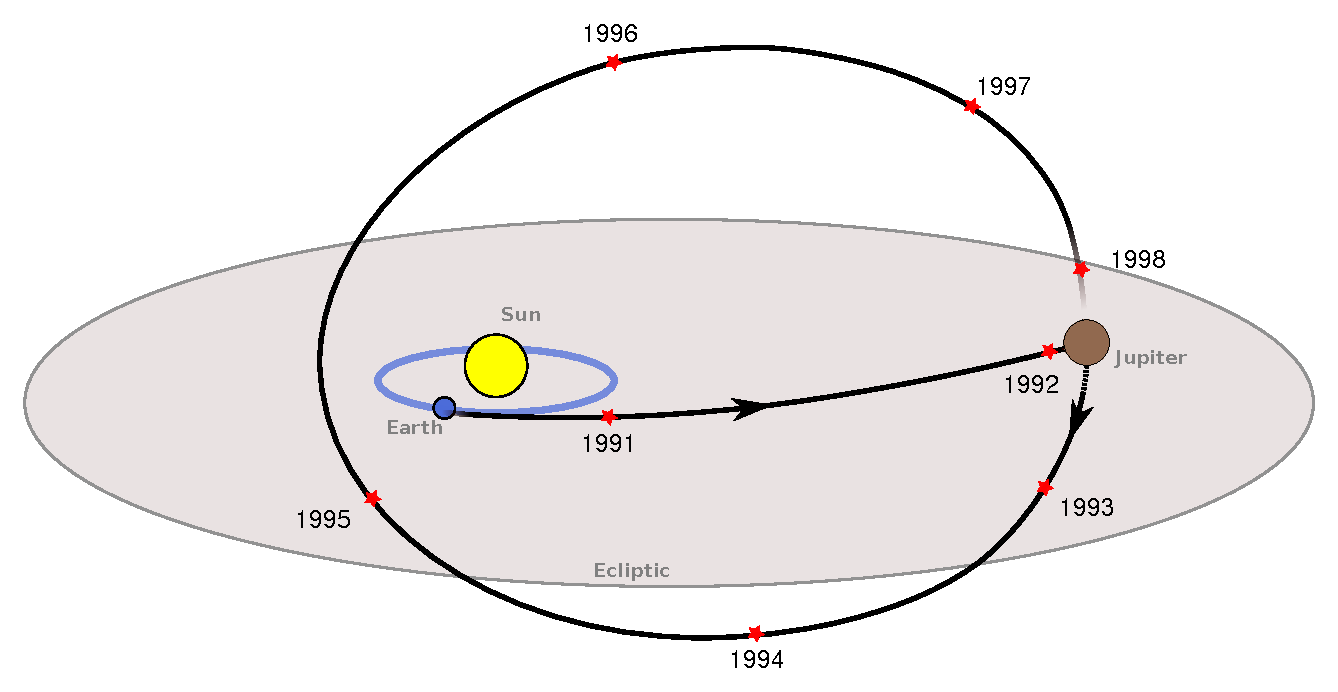
\includegraphics[width=0.8\textwidth]{Figures/ulysses_trajectory.pdf}
	\centering
	\caption{A sketch of Ulysses' first orbit. After the launch from earth in 1990 the spacecraft was sent to Jupiter from where it left the ecliptic on an elliptical orbit around the sun with perihelion at $1.3\,\mathrm{AU}$ and aphelion at $5.4\,\mathrm{AU}$. Due to the orbit's high latitude of $\sim 80 \, ^\circ$ Ulysses crossed the Sun's pole regions two times between 1994 and 1996. Figure after \citet{esa_orbit}.}
	\label{fig:trajectory}
\end{figure}
%
%
%
%
%
\section{SWICS}
\label{sec:swics}


\begin{figure}
	\centering
	\begin{subfigure}{.5\textwidth}
		\centering
		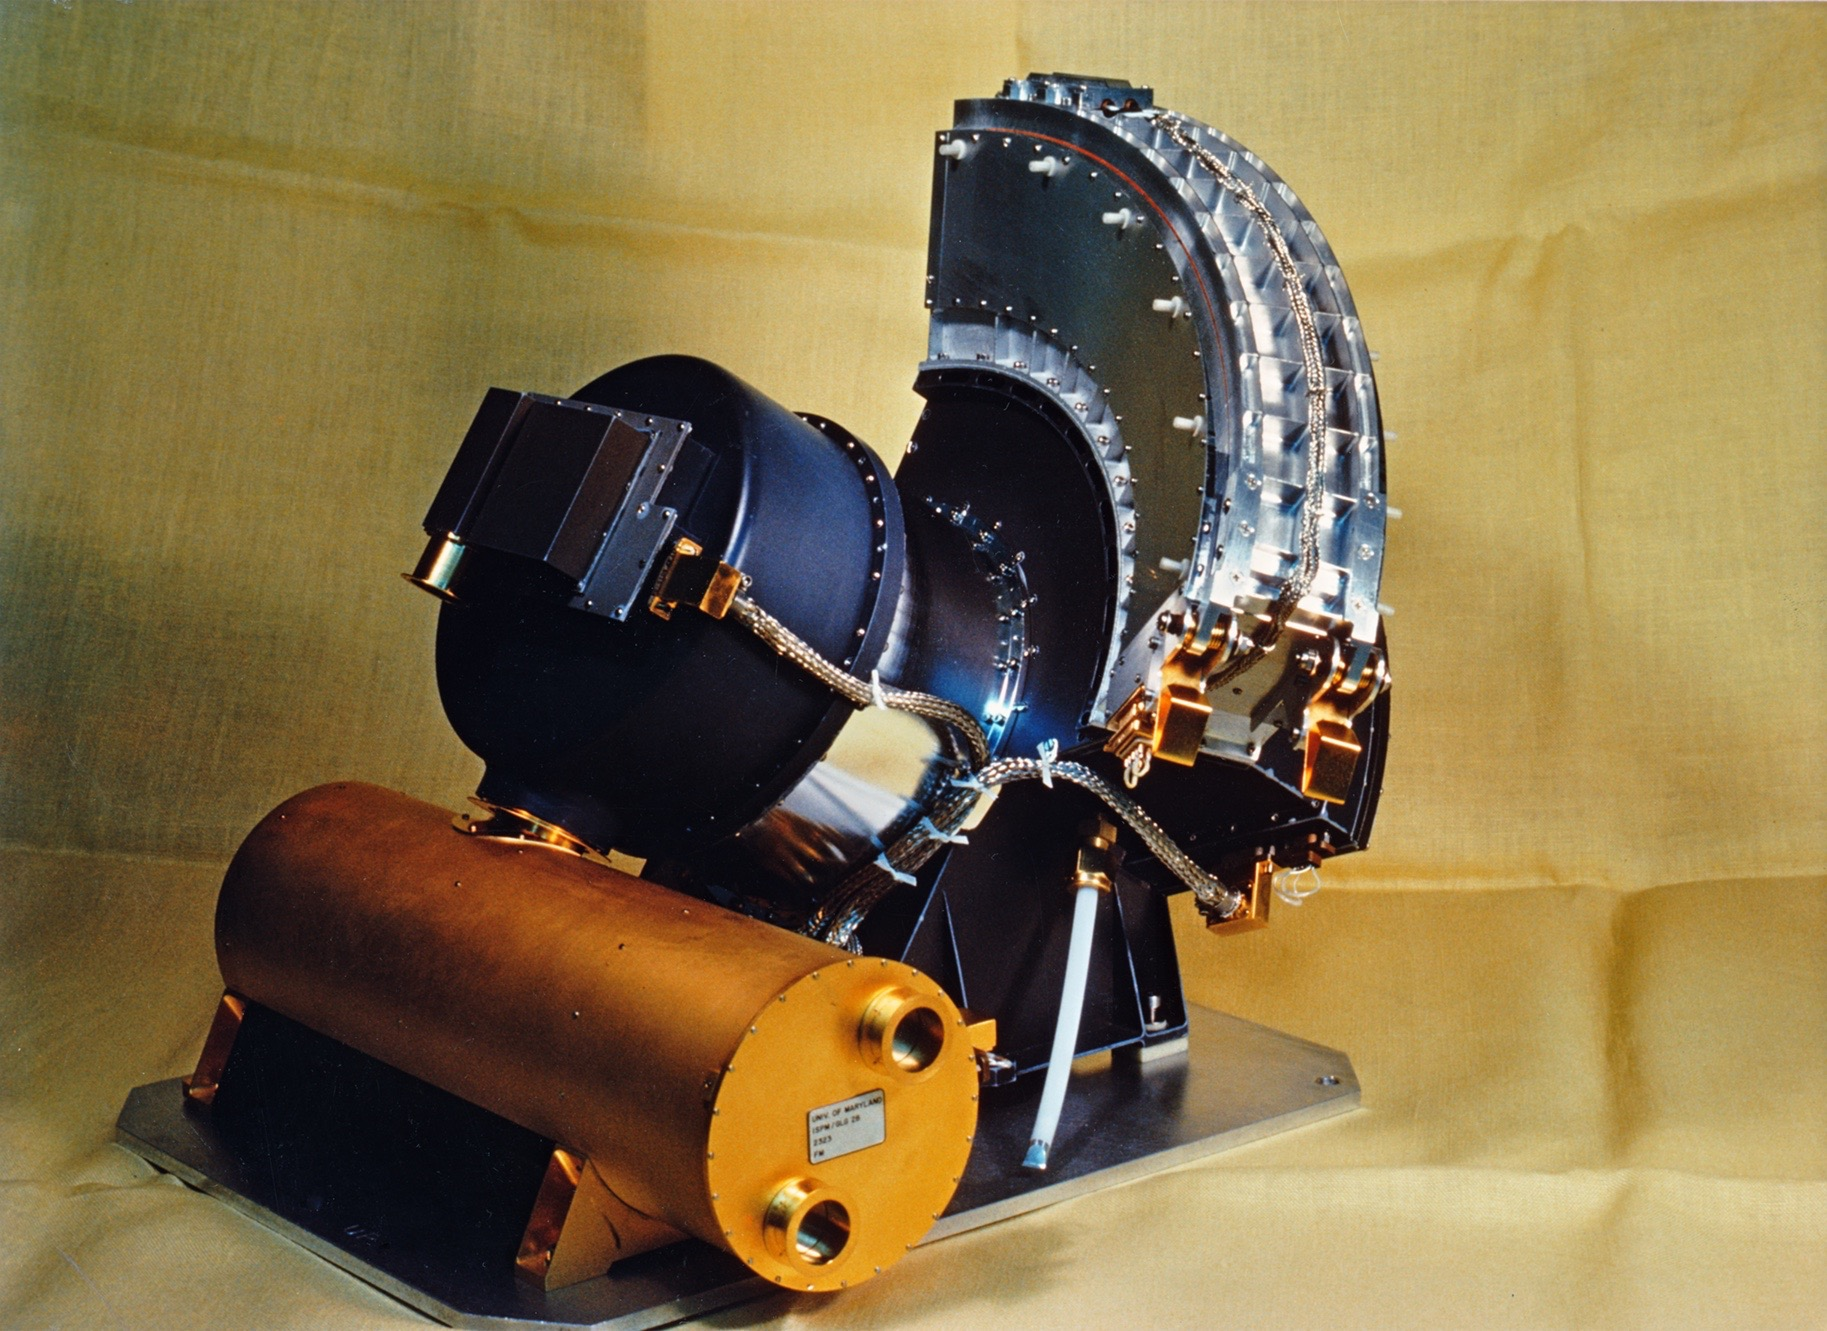
\includegraphics[width=0.9\linewidth]{Figures/ULYSSES-SWICS.jpg}
	\end{subfigure}%
	\begin{subfigure}{.5\textwidth}
		\centering
		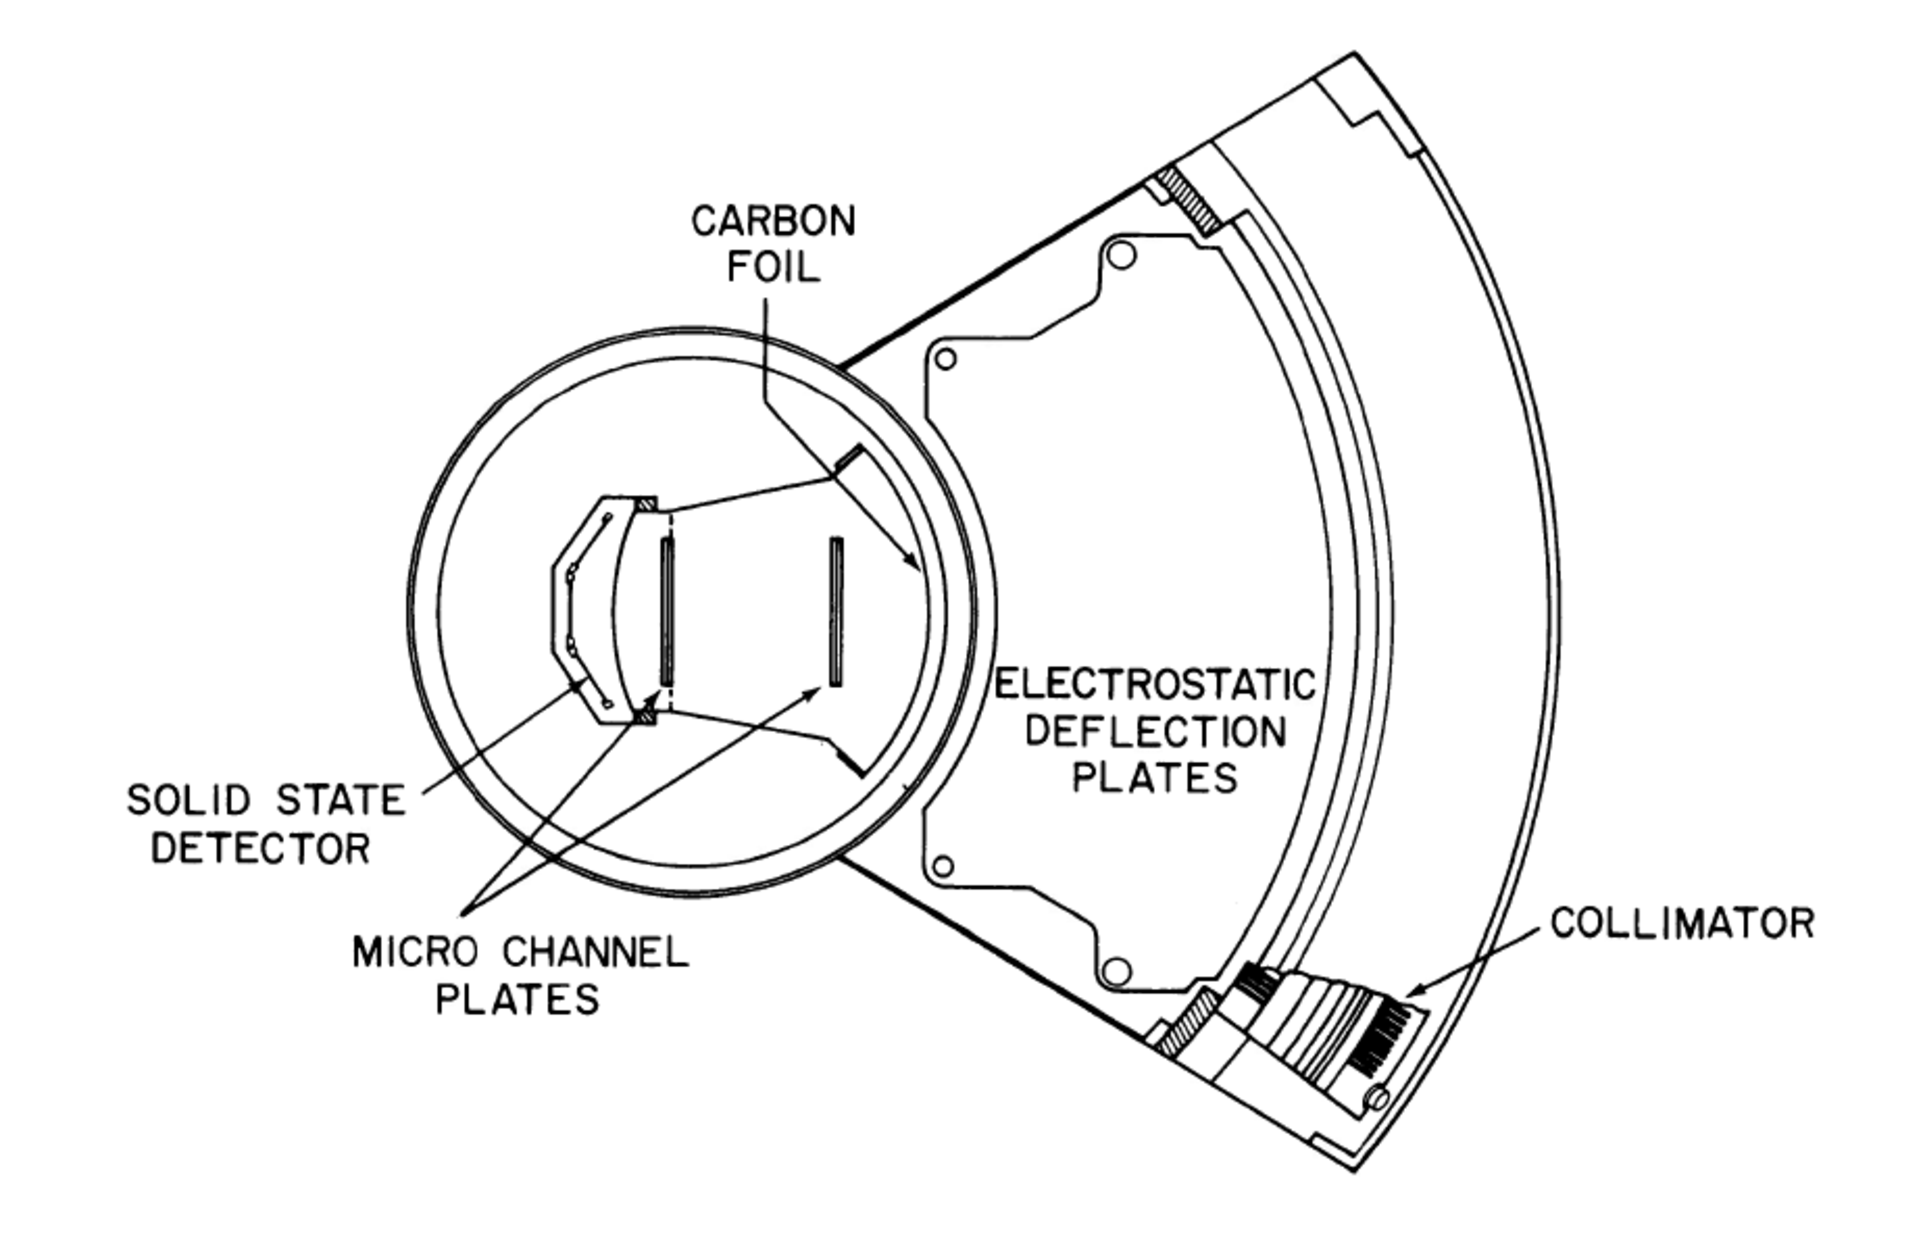
\includegraphics[width=1.1\linewidth]{Figures/swics_sensor.pdf}
	\end{subfigure}
	\caption{\\ \textit{Left:} Photograph of the SWICS instrument. The fan-shaped collimator on top of the electrostatic deflection analyzer can bee seen on the right. It is followed by the cylindrically shaped and silvery coloured \textit{high-voltage bubble}, that contains the time-of-flight system, analog electronics and and the sensor power supply. The gold-plated cylinder houses a $-30\,\mathrm{kV}$ voltage supply. The opening angles of the collimator are $69^\circ$ in width and $4^\circ$ in height. OPT: Ausschneiden und beschriften \\ \textit{Right:} Schematic cut through the sensor. In this view the orientation of the three solid state detectors is visualized. OPT: farbig markieren\\ Both figures are from from \citet{gloeckler_1992}.}
	\label{fig:swics}
\end{figure}

The Solar Wind Ion Composition Spectrometer (SWICS, \citet{gloeckler_1992}) is a time-of-flight mass spectrometer mounted on the spacecraft Ulysses (s. sec. \ref{sec:ulysses}). The instrument is designed to determine the elemental and charge-state composition and the velocity distribution of solar wind ions. With an energy-per-charge range from $0.16 \, \mathrm{kV}$ to $59.6 \, \mathrm{kV}$ SWICS is able to measure every solar wind ion species from protons to iron with any typical charge state. Depending on the individual ion, particle energies from $1 \,\mathrm{keV}$ up to $1 \, \mathrm{MeV}$ are covered.\\
SWICS is mounted on the sun-facing side of Ulysses and revolves around the spacecraft's spin axis with the spacecraft spinning. A photograph of the instrument is shown in fig. \ref{fig:swics}, left.\\
Ulysses SWICS also has a twin instrument that is the SWICS spare model, which has been mounted on the ACE spacecraft \citep{stone_ace}.
\\ \\ 
TODO: Super für measuring PUIs! viele wichtige Messungen... \\ \\
%
%
%
SWICS measures the mass $m$, the charge $q$ and the energy $E$ of entering ions by a combination of three separate measurements: The electrostatic deflection analyzer within the entrance systems is used for determining the energy-per-charge of a particle. Within the time-of-flight/energy section the particle's time-of-flight and residual energy are measured. A more detailed description of the measurement is given in the next sections. A particle's trajectory through the instrument can be tracked in the schematic in fig. \ref{fig:lars_swics}.
%
\subsection{Collimator and Electrostatic Analyzer}
\label{sec:EpQ}
Particles enter the instrument through the entrance collimator. It restricts particles to the ones with a trajectory that is parallel to the collimator slits.  The collimator follows an intricate geometry that is fan-shaped with an opening angle of $69^\circ$ in width and $4^\circ$ in height and that is at the same time curved along its width. Fig. \ref{fig:swics}, left,  gives an idea of the shape.\\
After having entered through the collimator a particle has to pass the electrostatic analyzer. It is split up into two sections -- energies-per-charge from $0.16$ to $14\,\mathrm{kV}$ are covered by the proton/helium channel. Particles within this range of energy will be filtered by their energy-per-charge and after an post-acceleration will be counted by a solid-state detector. As this simple measurement principle is very limiting for our analysis we will focus on the main channel that is suitable for a full \textit{mass/mass-per-charge} analysis.\\
The main channel covers an energy-per-charge range of $0.66$ to $60.51\,\mathrm{kV}$. A particle can only pass through the pair of curved deflection plates if its kinetic energy-per-charge equals a certain ratio that is given by the voltage between the two plates. To measure particles of different energy-per-charge the deflection voltage is stepped through 64 logarithmically spaced values, s. fig \ref{fig:epq}. As the voltage steps once per spin of Ulysses (every $12\,\mathrm{s}$), a complete voltage cycle lasts $\sim$ 12.8 minutes. 
Every step has a relative uncertainty in energy-per-charge of $\Delta \mathrm{EpQ / EpQ = 5\%}$  that is due to the finite space between the plates.
%
%
%
\begin{figure}[h]
	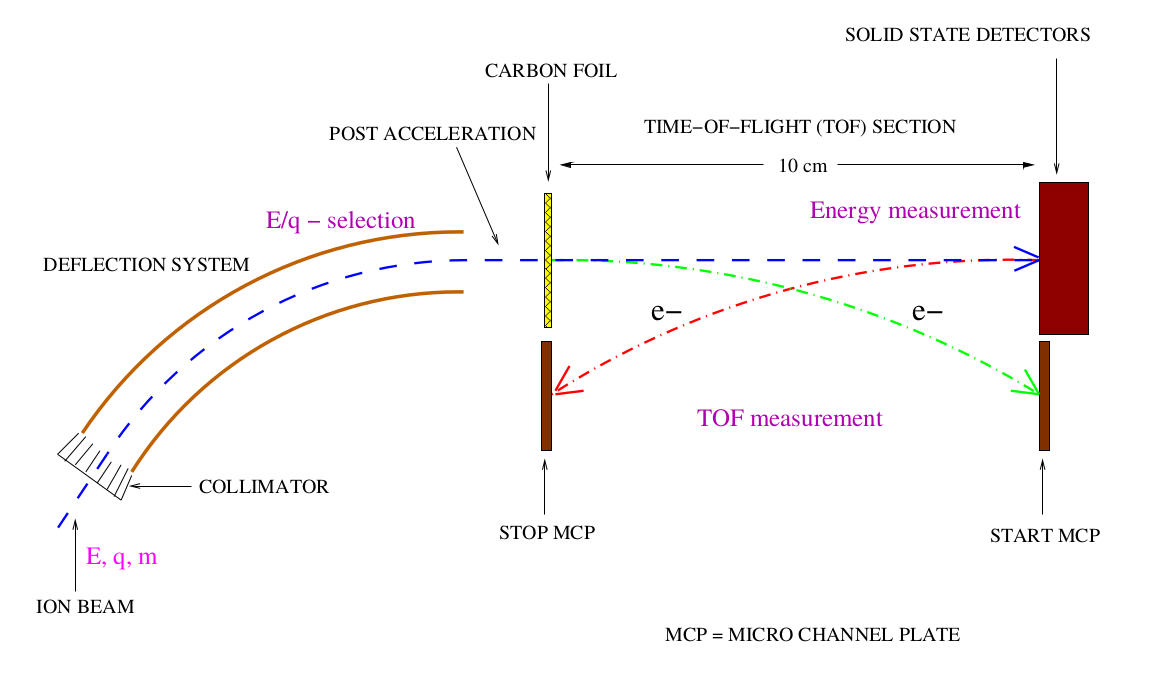
\includegraphics[width=0.8\textwidth]{Figures/Lars_Swics.png}
	\centering
	\caption{Schematic view of the SWICS detector. See text for reference. This figure is taken from \citet{lars-phd}.}
	\label{fig:lars_swics}
\end{figure}

%
\begin{figure}[h]
		\centering
		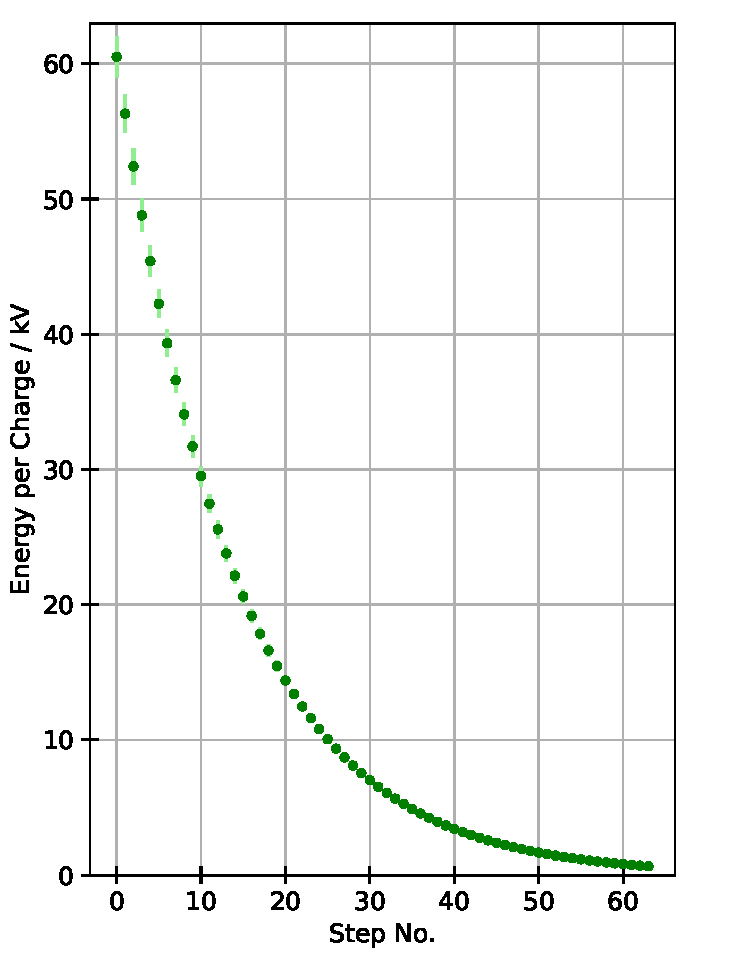
\includegraphics[scale = 0.7]{Figures/epq_err.pdf}
		\caption{Energy-per-Charge steps of Ulysses SWICS. A voltage cycle starts with step 0 that is the highest voltage $EpQ = 60.51\, \mathrm{kV}$. Voltage is then swept down 64 logarithmically spaced steps up to $EpQ = 0.66\, \mathrm{kV}$. The uncertainty of the single steps is $\frac{\Delta EpQ}{EpQ} = 5\%$ and drawn in lighter color.
		} \label{fig:epq}
\end{figure}
%
%
%
\subsection{Time-of-flight measurement}
After having passed the electrostatic analyzer the ion is post-accelerated by an constant potential drop of ~$30\,\mathrm{kV}$. It enters the time-of-flight chamber with penetrating through a thin ($\sim 3\,\mu \mathrm{g / cm^2}$) carbon foil from which secondary electrons are emitted. These electrons are guided to a microchannel plate detector where a start signal is triggered (s. fig \ref{fig:lars_swics}). The stop signal is triggered after the ion has traversed nearly force free a distance of $10\,\mathrm{cm}$ through the vacuumized time-of-flight section. Here it hits one of the solid-state detectors, where secondary electrons are emitted again. By combining the times of the start and the stop signal the particle's time-of-flight has been measured.
\subsection{Energy measurement}
Additionally, the ion's energy is measured when they hit one of the three solid state detectors. \\
A solid-state detector is realized by applying an inverse bias voltage to a semiconductor material. When ionized particles hit the material, they set free charge carriers from the resulting depletion zone. These charge carriers can be measured as a pulse of current which is proportional to the deposited energy of the ion. \\
Each of the three detectors has an active area of $1.5 x 1.3 \,\mathrm{cm^2}$. Their alignment with each other can be seen in fig \ref{fig:swics}, right: While the central detector is oriented perpendicular to the symmetry axis of SWICS, the other two detectors are slightly tilted with respect to this axis. This way particles with different angles of incidence along the width of the collimator can be detected. The information on which of the three detectors has been hit will be utilized in chapter \ref{chapter:data} for a coarse directional resolution of incident particles.
\\ \\
One of SWICS' main objectives is the measurement of the composition of incident particles. An ion and its charge state can be fully identified with the knowledge of its mass $m$ and its mass-per-charge $mpq$. 
With the measurement of the time-of-flight $ToF$, the energy $E_{SSD}$ and the knowledge of the energy-per-charge $EpQ$ we can calculate the mass $m$, the mass-per-charge $mpq$ and velocity $v$ of an ion $i$ with the following set of equations:
\begin{align}
m_i &= 2\,E_{SSD} \left( \frac{Tof}{d}\right)^2 \label{eq:swics_set1}\\
mpq_i &= 2 \left(EpQ + V_{PAC}\right) \cdot \left(\frac{Tof}{d}\right)^2 \label{eq:swics_set2} \\
v_i &= \sqrt{2\,EpQ\,\frac{1}{mpq_i}},
\label{eq:swics_set3}
\end{align}
where $d$ is the length of the time-of-flight section and $V_{\mathrm{PAC}}$ is the post-acceleration voltage. $v$ denotes the ion's initial velocity when entering the instrument and is not to be confused with its velocity during the time-of-flight measurement, that is altered particularly by the post-acceleration.
%
%
%
\section{Data products}
\label{sec_dataprod}
Direct Pulse-Height Analysis data (PHA data) are one of SWICS' data products and the ones that are most relevant for the analysis in this work.\\
Over one voltage cycle SWICS steps through the 64 energy-per-charge steps of the electrostatic analyzer (s. sec \ref{sec:EpQ}), which we call ESA steps. At normal spacecraft telemetry rates SWICS steps once per spin, which is once every $12\,\mathrm{s}$. During these times 30 PHA words per spin are selected and transmitted. The selection is based on a priority scheme that is described below in sec. \ref{subsec:prio}.\\
Every 24-bit PHA word contains following information on an incident particle that triggered a valid measurement:
\begin{itemize}
	\item $E_{SSD}$: Energy deposition in the solid state detector \\
	measured through 256 channels in a range $40 - 600\,\mathrm{keV}$
	\item $ToF$: Time-of-Flight\\
	measured through 1024 channels in a range $10 - 200\,\mathrm{ns}$
	\item Sector information:\\
	SWICS divides one spin of Ulysses up into 8 sectors of approximately equal duration. This yields in information on the spatial origin of particles.
	\item Detector information: \\
	Which of the three solid state detector elements has been triggered?
	\item Priority category: \\
	Due to limited telemetry only an assorted sample of all measured particles can be transmitted. This selection is based on different priorities. For details s. sec \ref{subsec:prio}.
\end{itemize}
The interpretation of a set of PHA words that have been collected over time is discussed in sec. \ref{sec:etmatrices}. 
%
\subsection{Detection Efficiency}
\label{subsec:det_eff}
When working with SWICS -- like for any physical measurement -- one has to consider several constraints that impede the ideal measurement as it is described in sec. \ref{sec:swics}. \\
One of these constraints is the detector efficiency, which describes the probability to measure a particle that has entered the instrument (Todo: ?). 
With an ion passing through the time-of-flight section there is the likelihood that secondary electrons may not be emitted properly from the carbon foil and solid state detector which then leads to an invalid time-of-flight measurement. Also, ions could pass through the time-of-flight section on divergent trajectories due to scattering processes (TODO: in the carbon foil??). Subsequently, the ion possibly does not hit the sensitive area of the solid state detector and would neither trigger a stop signal for the time-of-flight measurement nor a valid energy measurement in the solid-state detector.\\
Another reason for an invalid energy measurement in the solid-state detector can be that the ion's energy is smaller than the threshold of the solid-state detector. In this case, only energy-per-charge and time-of-flight information for the ion are available. Such events without a corresponding energy measurement are called double coincidences, while events with triggered start and stop signal and an energy measurement are called triple coincidences.\\
The reason for choosing a non-zero threshold is to limit the influence of the solid-state detector's natural noise. For SWICS this noise level is quite high, at around $12\,\mathrm{keV}$ \citep{gloeckler_1992} (todo: ?), so that the threshold is chosen to be $\sim 30 \, \mathrm{keV}$. 
The detection efficiency is highly dependent on the ion species and deflection step.
Ions with a small mass and charge are most likely to not overcome the threshold at low energy-per-charge values. For the bulk of $\mathrm{He^{+}}$ this is already the case for ESA step 17 ($EpQ = 17.86\,\mathrm{kV}$), which corresponds to a $\mathrm{He^{+}}$ velocity of $v = 900\,\mathrm{km\,s^{-1}}$ (s. eq. \ref{eq:swics_set3}).\\
Unfortunately, $\mathrm{He^{+}}$ detection efficiencies are not known to us for Ulysses SWICS. Instead, we make use of the efficiencies from ACE SWICS, that have been calculated by \citet{koeten}. As ACE SWICS uses different energy-per-charge ranges we had to extrapolate the values for Ulysses SWICS.
For the highest energy-per-charge value $EpQ = 60.51\,\mathrm{keV}$ we interpolated the efficiency from the ACE $\mathrm{He^{+}}$ triple efficiencies and then extrapolated linearly to an efficiency of 0 at ESA step 17. By this, we accommodate for the above mentioned fact that $\mathrm{He^{+}}$ does not have enough energy to deposit energy above the solid state detector's threshold at ESA step 17 and thus, the probability for a triple coincidence is zero. $\mathrm{He^{+}}$ efficiencies from ACE SWICS and the resulting efficiencies used for Ulysses SWICS are shown in fig. \ref{fig:guess_eff}. For sure, these values are not realistic but represent the overall trend of a decreasing efficiency for higher ESA steps.
\begin{figure}[h]
	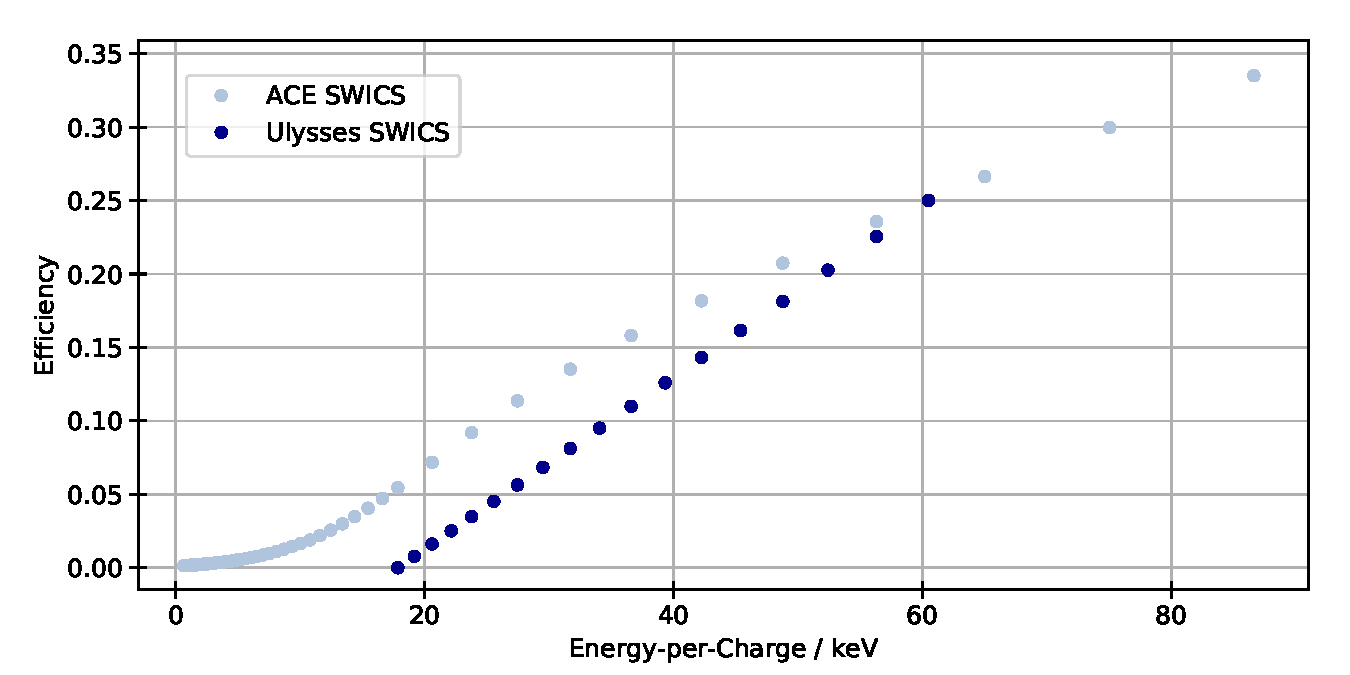
\includegraphics[width=1.\textwidth]{Figures/guess_eff.pdf}
	\centering
	\caption{$\mathrm{He^{+}}$ detection efficiencies for ACE SWICS over all ESA steps from $0.66\,\mathrm{kV}$ to $86.64\,\mathrm{kV}$. For Ulysses SWICS the efficiencies have been extrapolated between 0 for ESA step 17 ($EpQ = 17.86\,\mathrm{kV}$) and the highest efficiency for ESA step 0 ($EpQ =60.51\,\mathrm{kV}$). The latter value has been interpolated from the ACE efficiencies.}
	\label{fig:guess_eff}
\end{figure}


\subsection{Priority Weighting}
\label{subsec:prio}
SWICS' data processing unit performs an on-board mass and mass-per\--charge-clas\-sification. For every ion with valid measurements the mass $m$ and mass-per-charge $mpq$ are calculated based on the measurements of $E_{\mathrm{SSD}}$, $ToF$ and the particle's ESA step using a look-up-table technique.\\
On the one hand these values are used for sorting the ions into predefined boxes in the $m$-$mpq$-space which yield in the so-called matrix rate, a second data product that is provided benath the PHA words.\\
Secondly, and more important for our analysis, the m and mpq information is used to sort every measured ion into one of three priority ranges. Due to a limited telemetry possibly not every measured particle can be transmitted as a PHA word. 
30 PHA words per spin are chosen from these ranges in way that the ratio of low and high priority PHA words is balanced. By this selection less abundant heavier ions are artificially enhanced which is necessary to recreate the measured composition from the transmitted PHA words. Table \ref{tab} shows a summary of this priority scheme. Details about this can be found in \citet{gloeckler_1992}.\\
To account for the priority biased selection of PHA words it is necessary to weight the transmitted data with the so-called base-rate weight $brw = \frac{D_{\mathrm{PHA}}}{T_{\mathrm{PHA}}}$, where $T_{\mathrm{PHA}}$ is the number transmitted PHA words and $D_{\mathrm{PHA}}$ the number of detected particles on which this PHA word is based. The measured composition can be restored in this way.
\begin{table}[h]
	\caption{SWICS' priority categorization scheme} 
	\centering
	\begin{tabular}{c|c|c}
		%\hline
		Range 0 & $m < 8.7$;  $m_0 : mpq < 3.3$ & $\mathrm{H}$, $\mathrm{He^+}$, $\mathrm{He^{2+}}$; Doubles\\ 
		\hline 
		Range 1 & $m > 8.7$ & Heavier ions \\ 
		\hline 
		Range 2 & $m_0 : mpq > 3.3$ & Doubles \\ 
		%\hline 
	\end{tabular} 
	\label{tab}
\end{table}
%
%
%
\section{ET matrices, identification}
\label{sec:etmatrices}
Fig. \ref{fig:et_matrix} shows longterm PHA data collected over two years with Ulysses SWICS for ESA step 24 ($EpQ = 10.8\,\mathrm{kV}$). For every particle with valid time-of-flight and energy measurements the $E_{\mathrm{SSD}}$ channel is plotted over the time-of-flight channel. As a particle's mass and mass-per-charge are connected to the measured values $EpQ$, $ToF$ and $E_{\mathrm{SSD}}$ by equations \ref{eq:swics_set1} --  \ref{eq:swics_set3}, every ion species occupies a distinct position in this histogram, which we call ET-matrix. 
However, due to uncertainties in the measurements of $EpQ$, $ToF$ and $E_{\mathrm{SSD}}$ an event may be displaced around its ideal position. 
For multiple events of the same species this results in broadened distributions. A detailed discussion on these uncertainties can be found for example in \citet{lars-phd}.
We can identify several ion species in the shown ET-matrix: A selection of those is labelled in \ref{fig:et_matrix}.



\begin{figure}[h]
	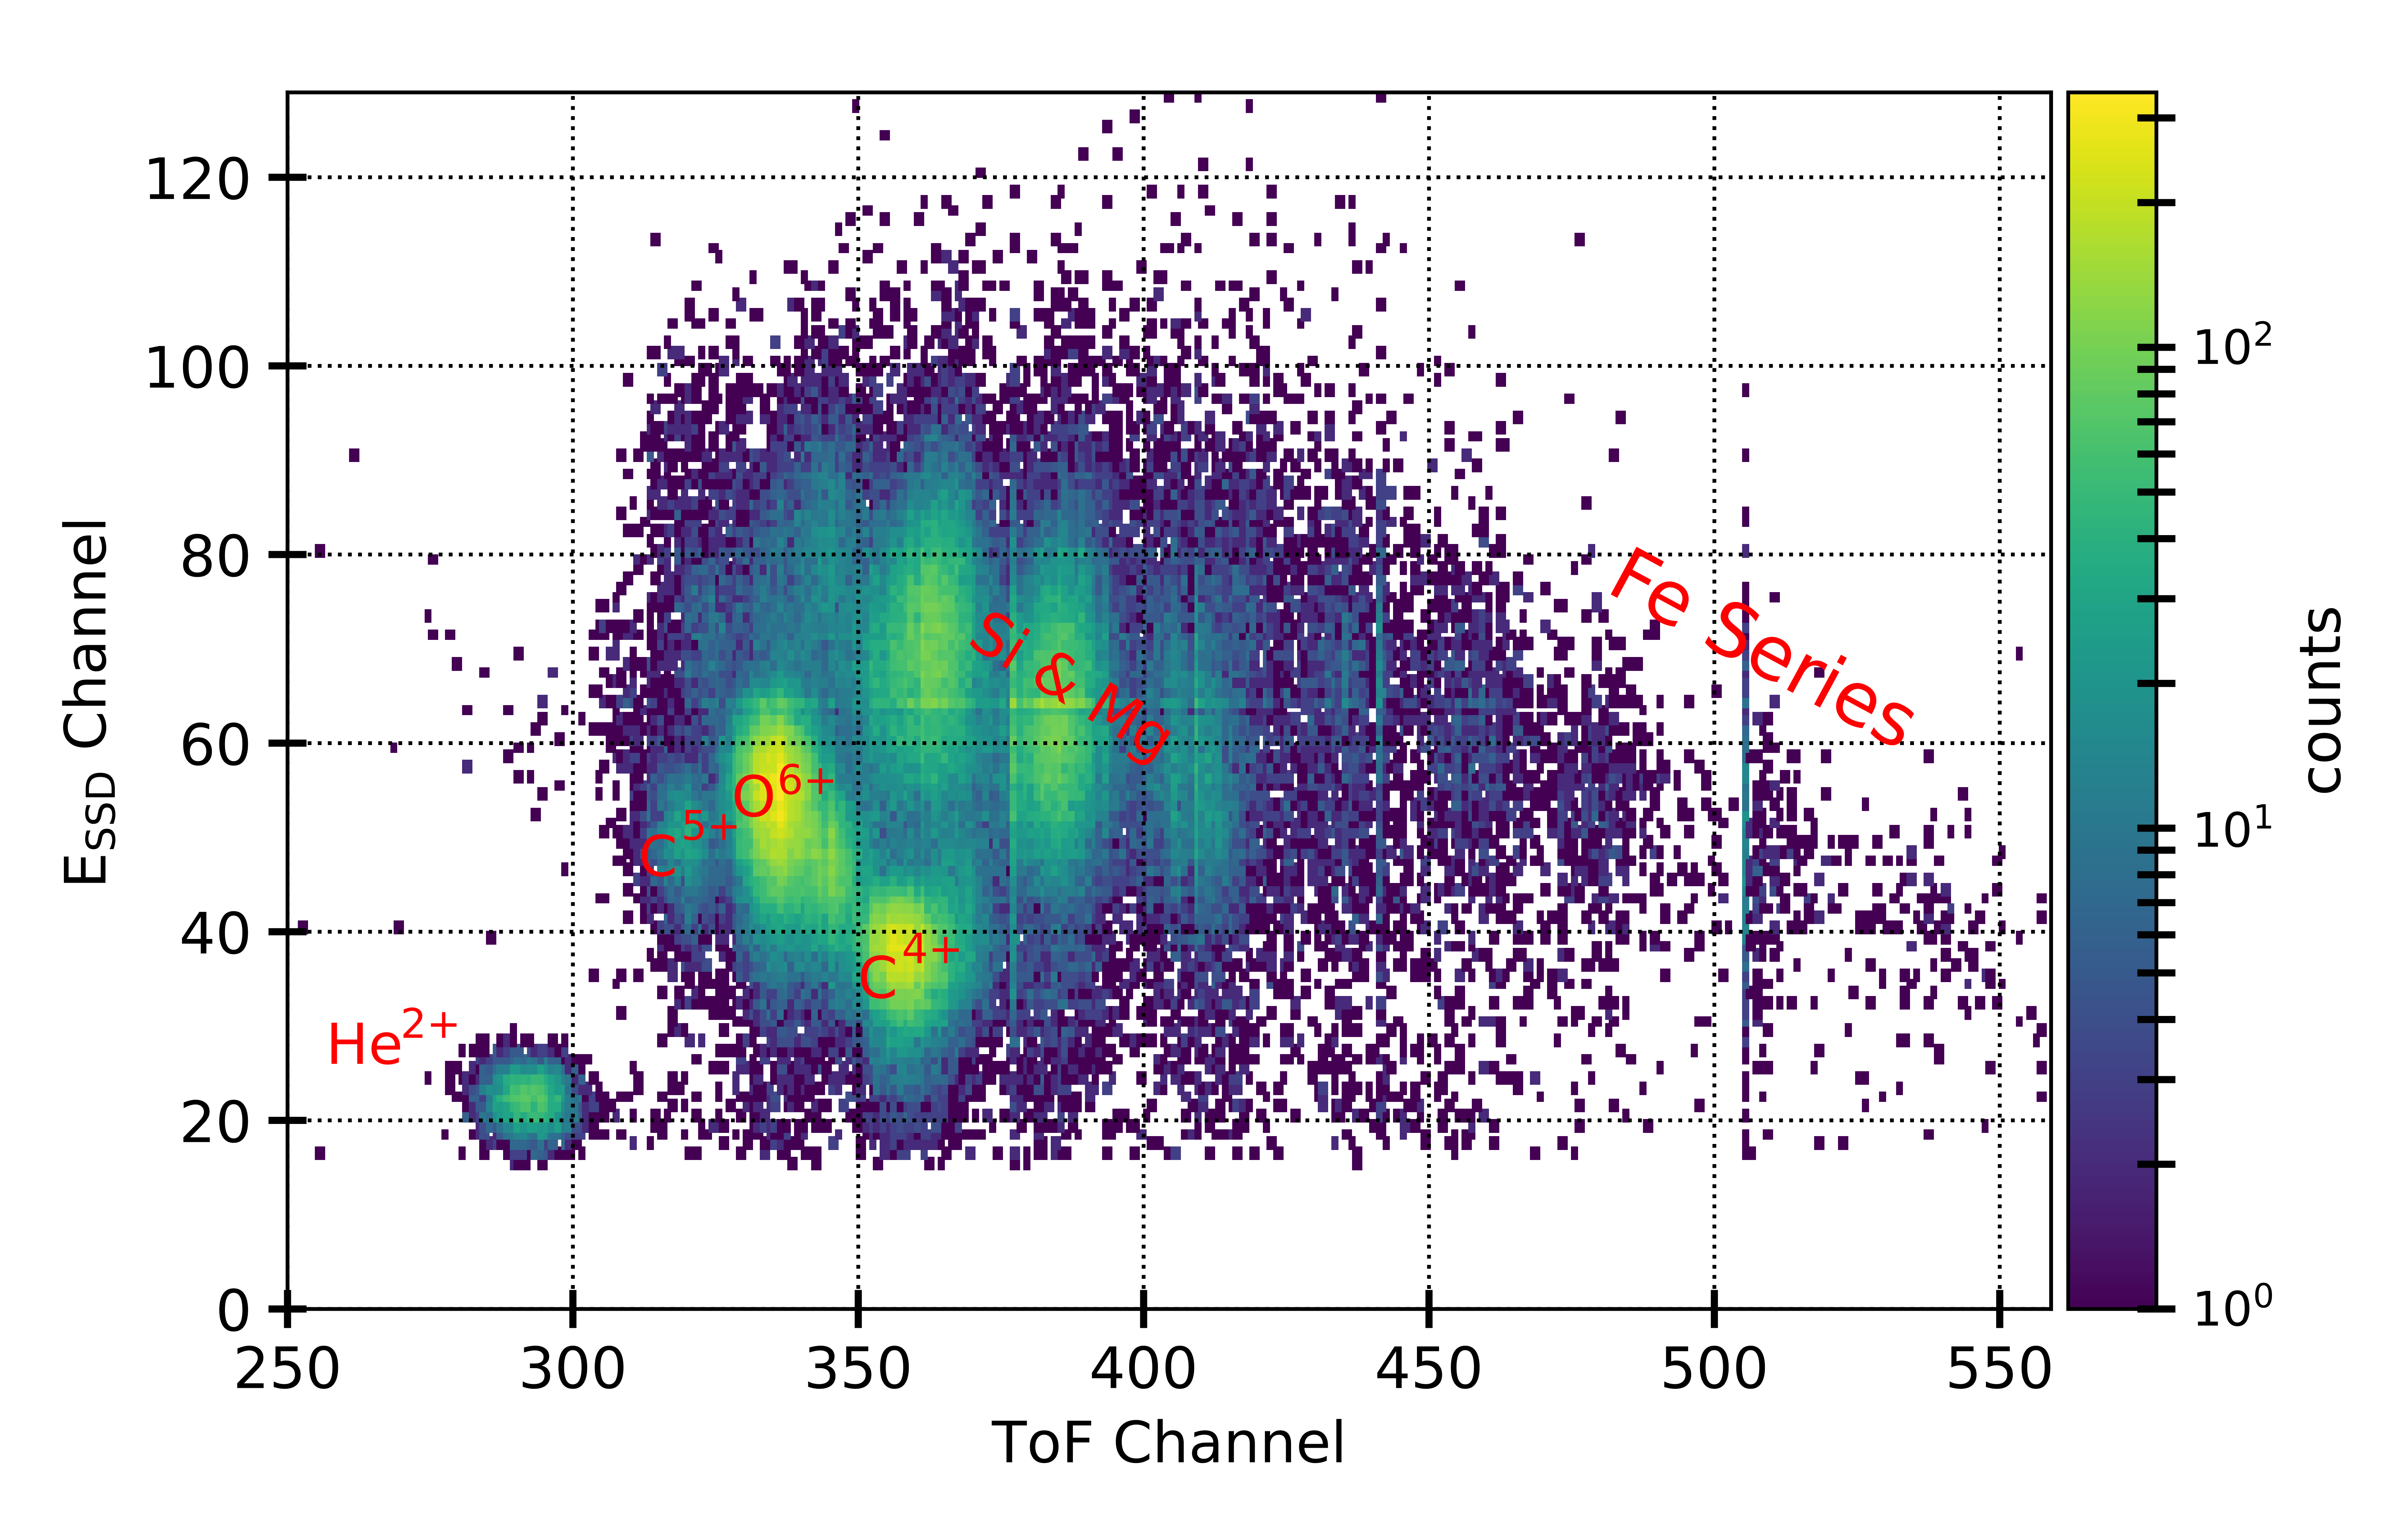
\includegraphics[width=0.9\textwidth]{Figures/et_matrix_labels.png}
	\centering
	\caption{ET-matrix from Ulysses SWICS PHA data of years 1993-1994. All plotted events were measured during ESA step 24 ($EpQ = 10.8\,\mathrm{kV}$). Only triple coincidences are shown. Besides accumulated counts in ion-specific positions, there are a few horizontal and vertical stripes apparent in the shown ET-matrix -- for example in $E_{SSD}$ channel 65 and time-of-flight channel 409, 377 or 505. These are imprints of irregularities within SWICS' Analog-Digital-Converters which can be noticed as a saturation of one bin while the adjacent bin is depleted. However, these signatures are not expected to have a significant effect on the following analysis.}
	\label{fig:et_matrix}
\end{figure}


\subsection{Selection of $\mathrm{He^{+}}$}

\begin{figure}[h]
	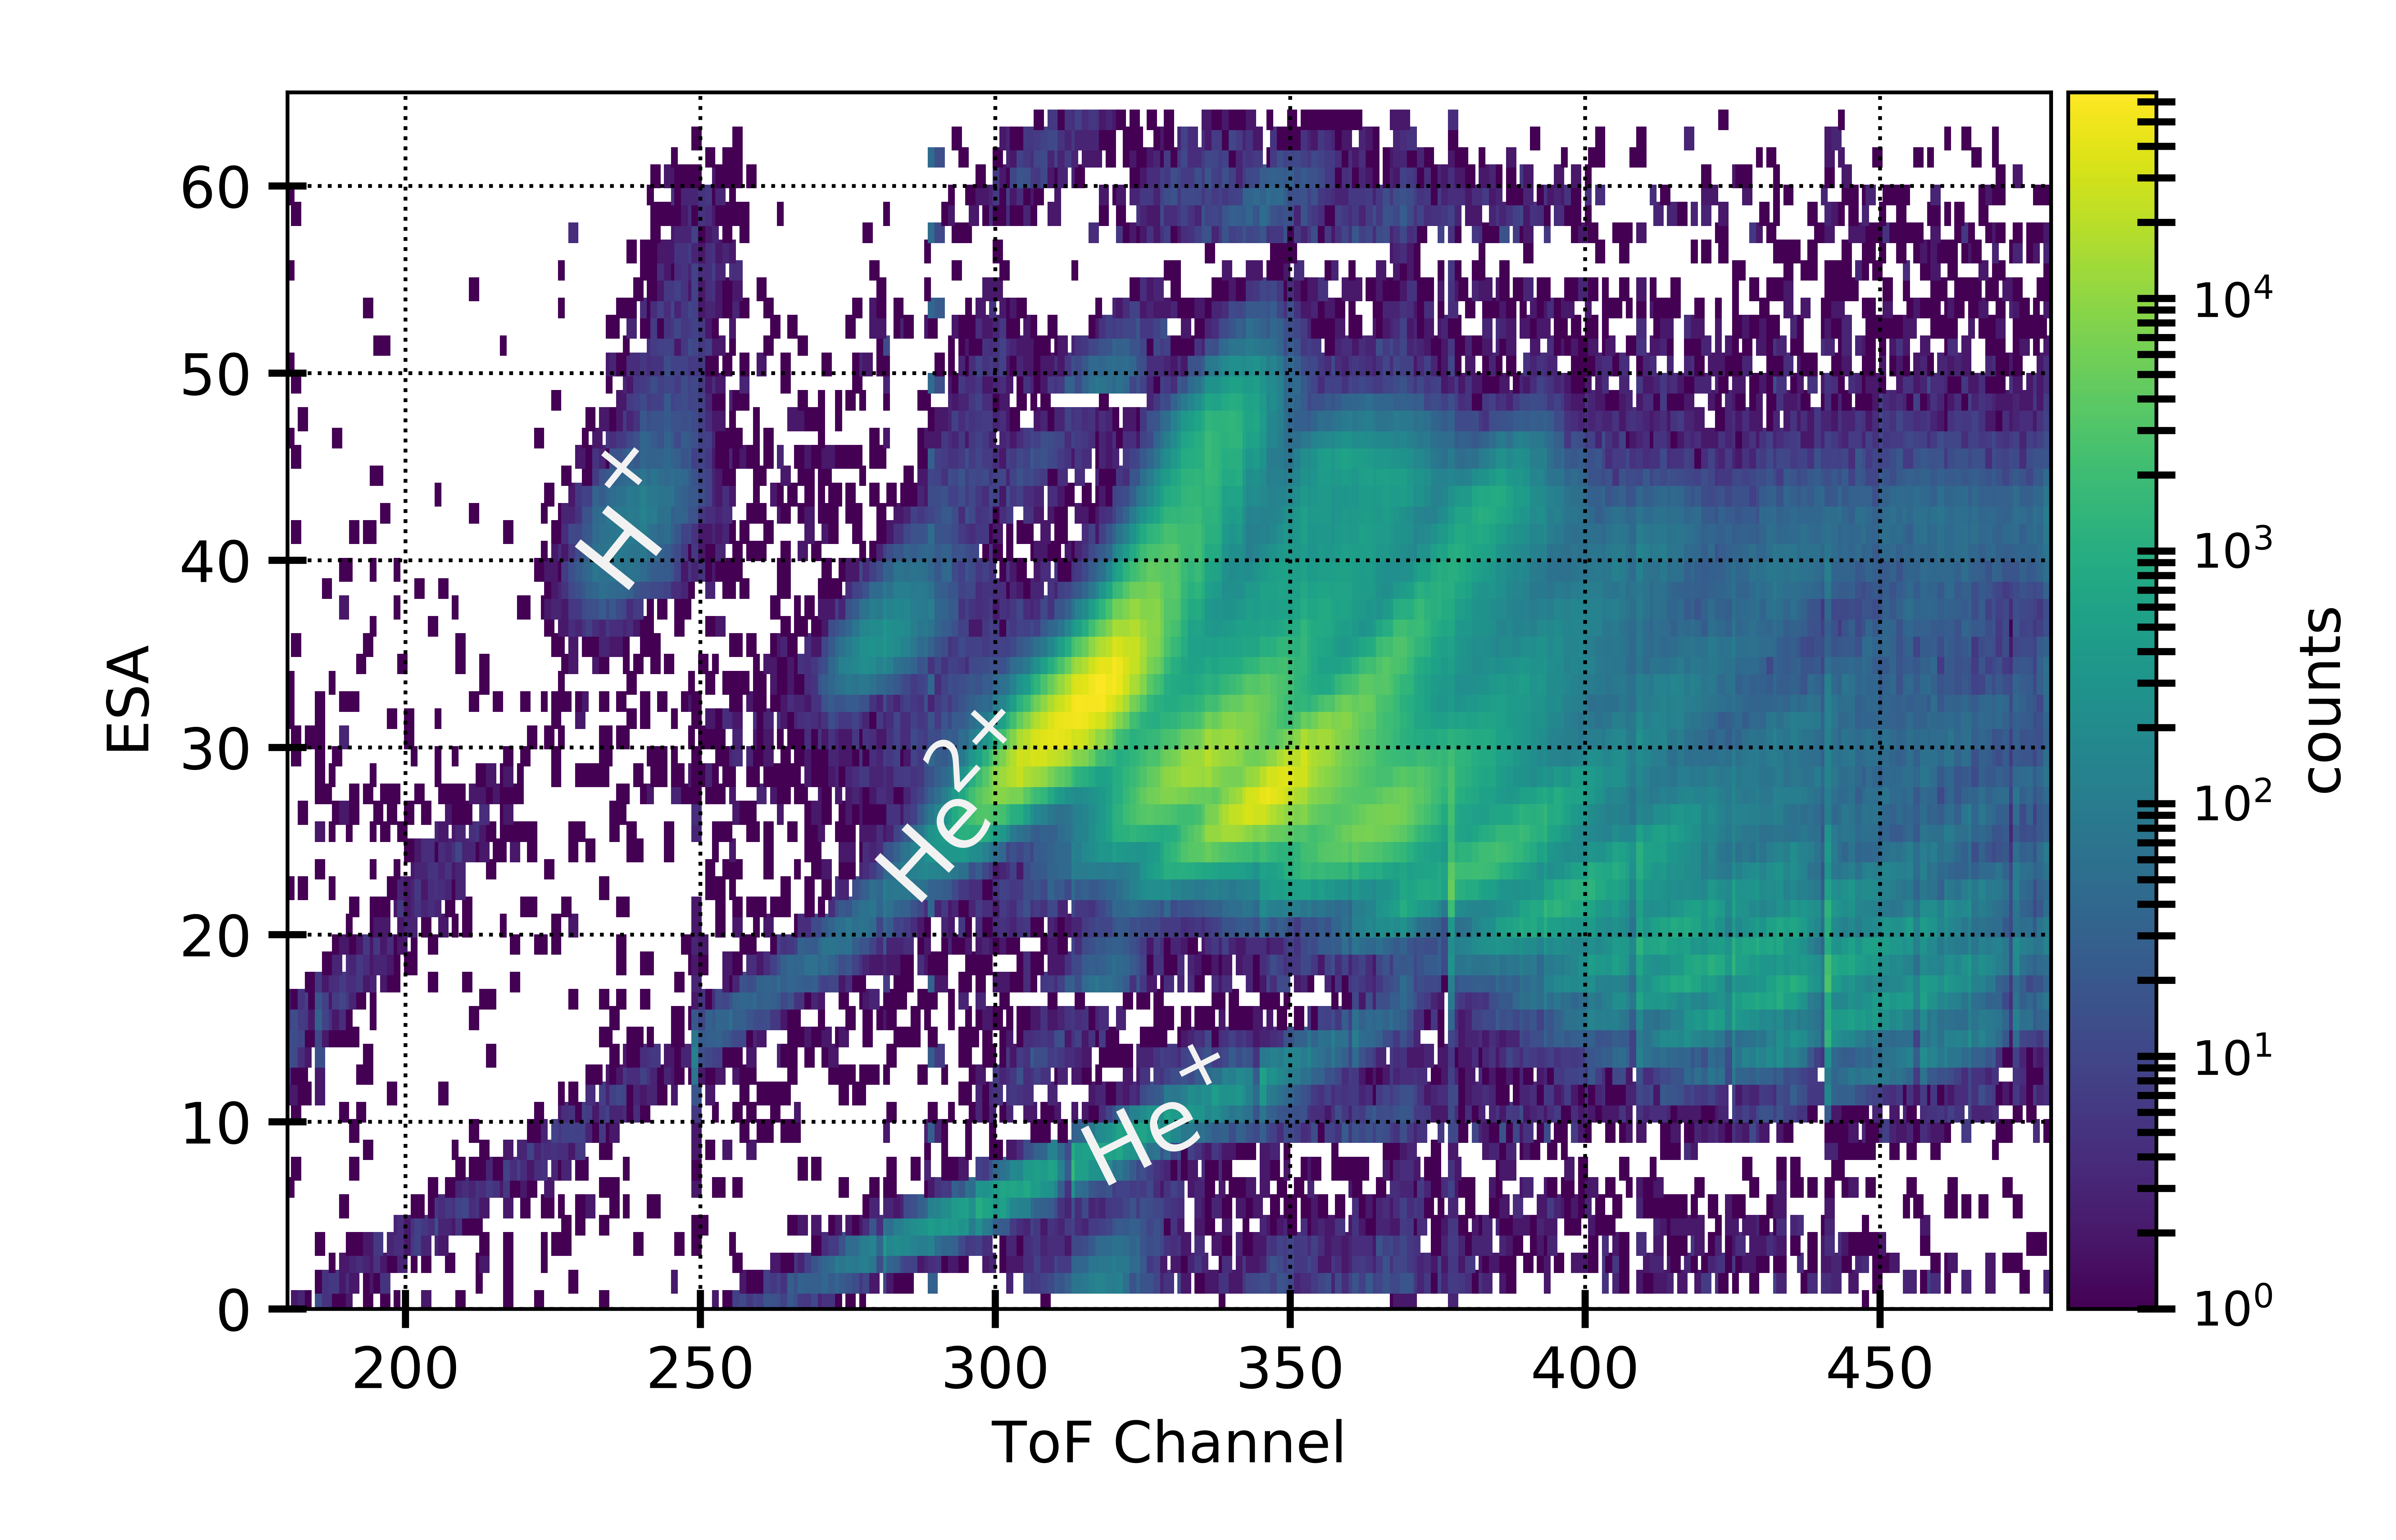
\includegraphics[width=0.9\textwidth]{Figures/epq_all.png}
	\centering
	\caption{Histogram over time-of-flight and ESA channels of two years (1993-1994) of Ulysses SWICS Triple Coincidence PHA data. Note, that the ESA channel numbers are inversely proportional to the energy-per-charge values. Ion species with the same mass-per-charge ratio can be detected on curves $ESA \sim ToF^2$.}
	\label{fig:epq_all}
\end{figure}

\begin{figure}[h]
	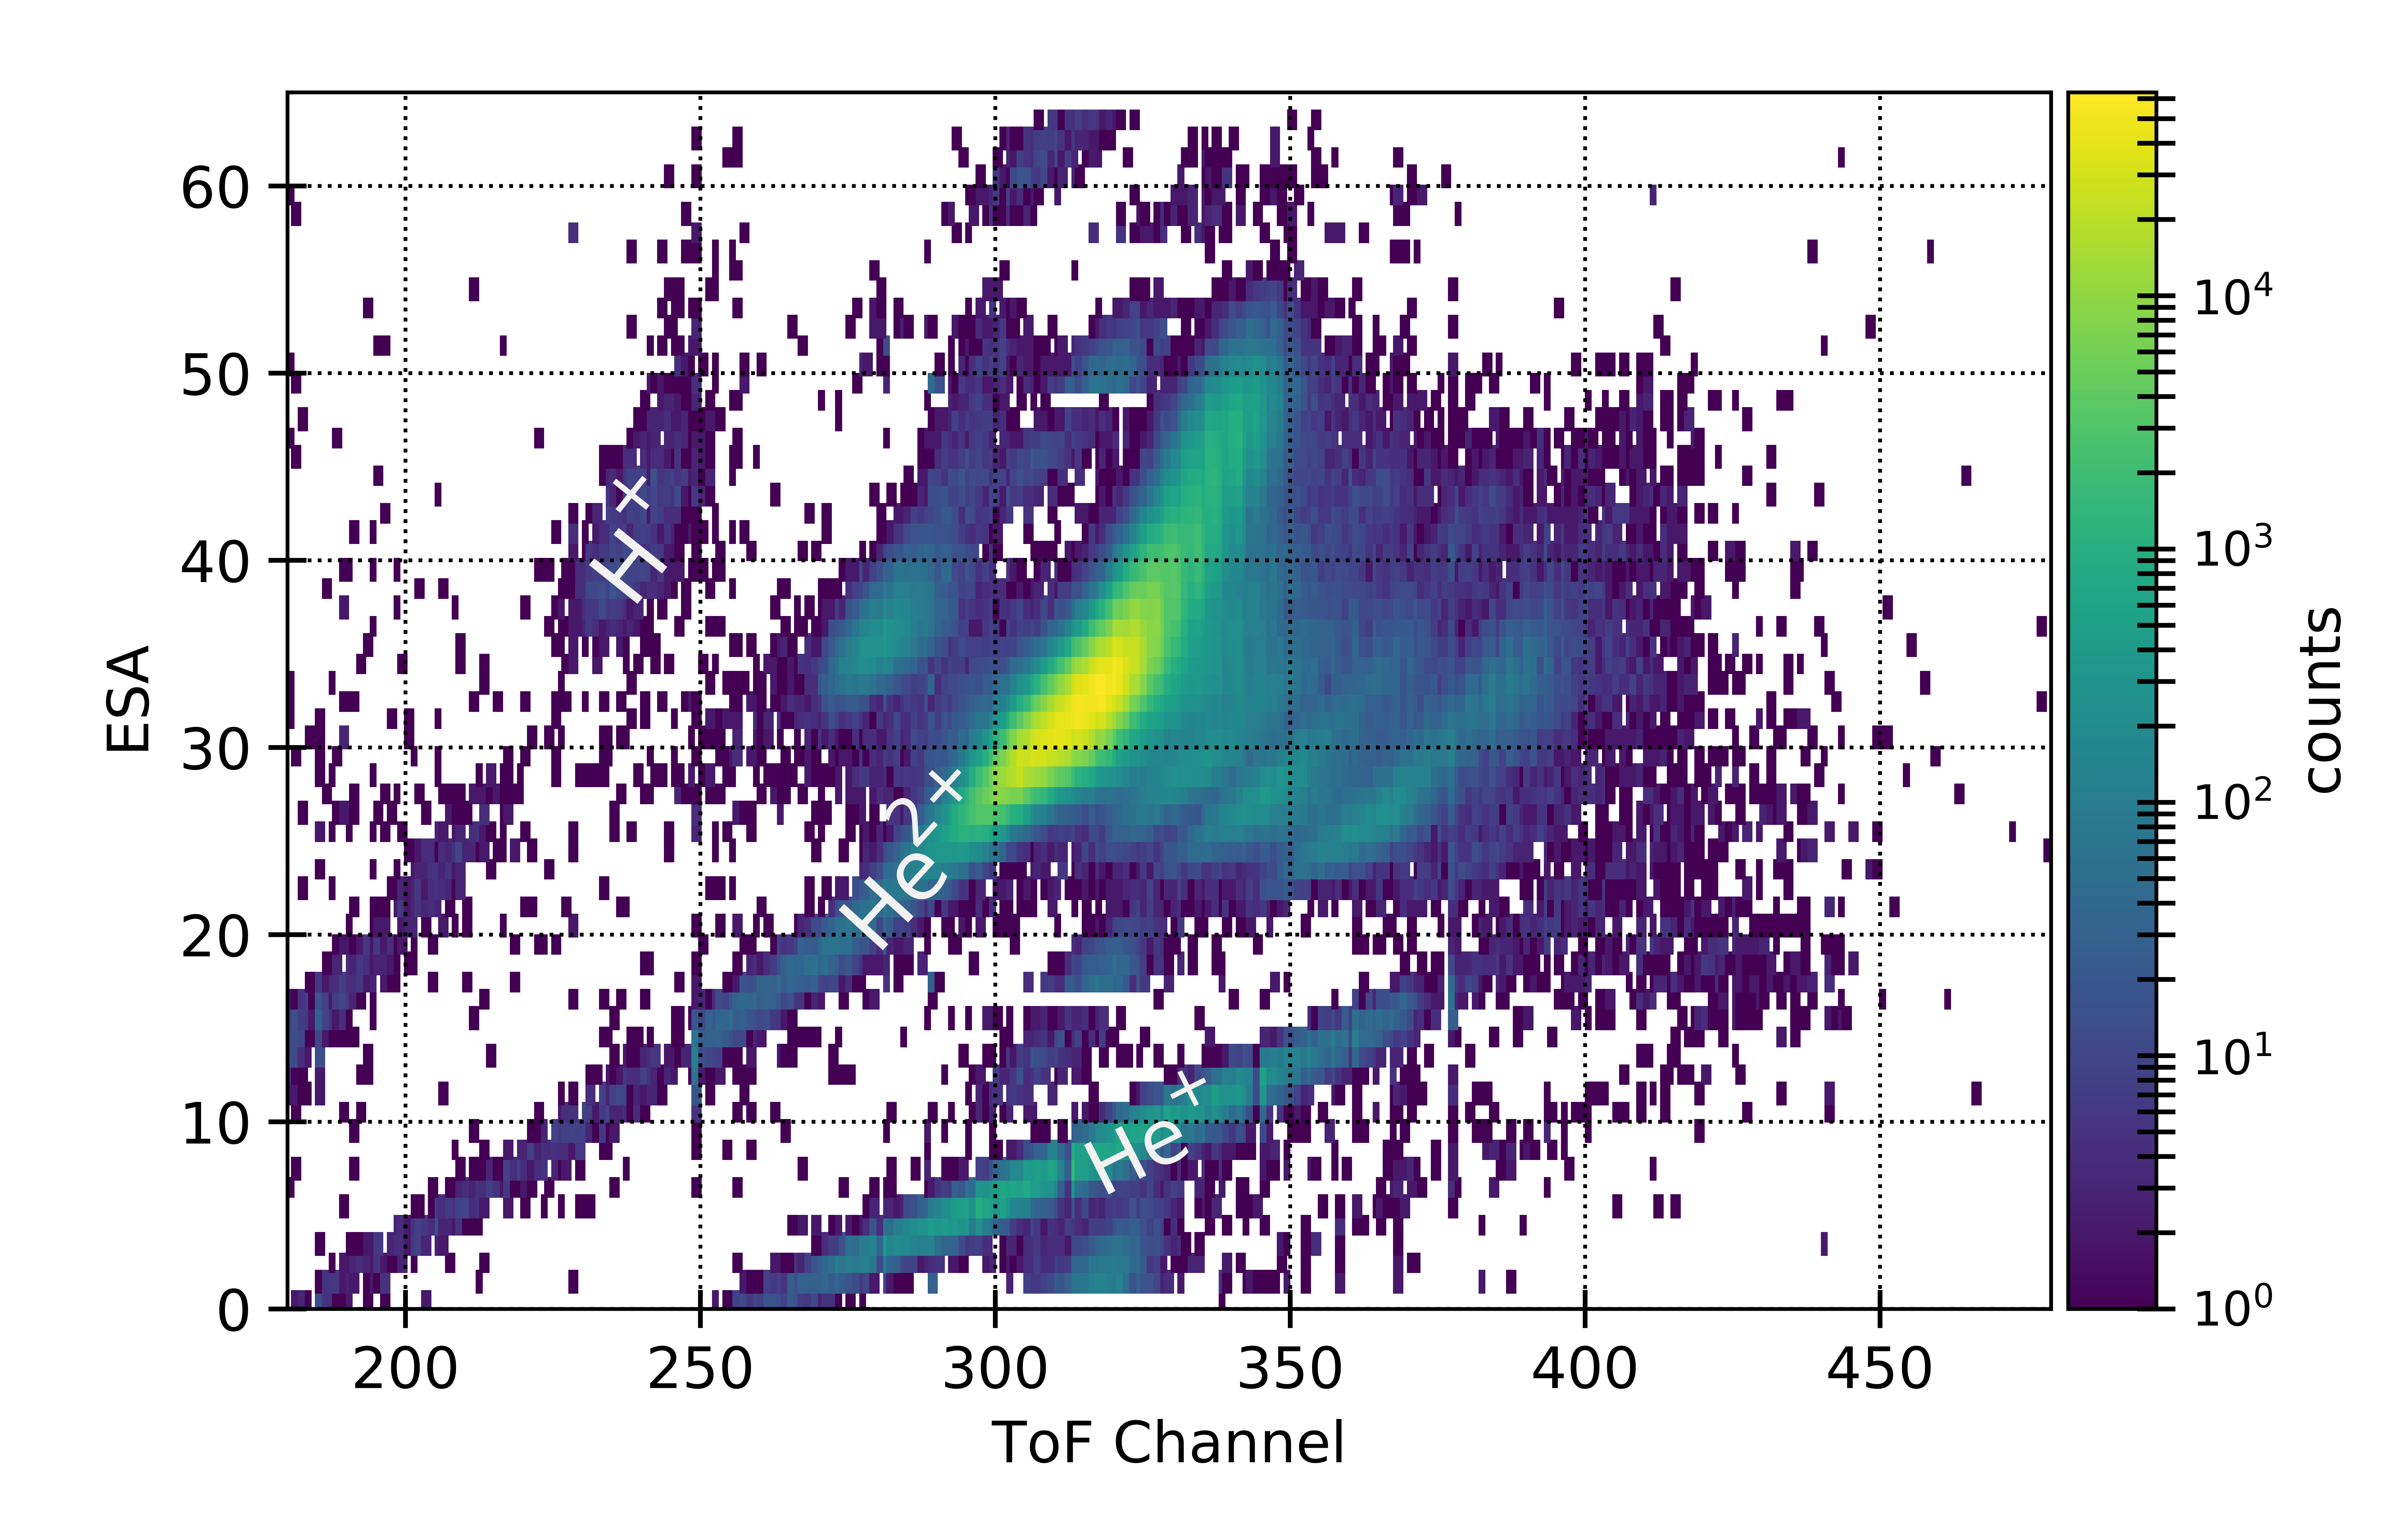
\includegraphics[width=0.9\textwidth]{Figures/epq_rng0.png}
	\centering
	\caption{The same histogram as in fig. \ref{fig:epq_all}, but this time only events with Range-0 priority are plotted. This basically removes ions with $m>8.7\,\mathrm{u}$.}
	\label{fig:epq_rng0}
\end{figure}


For extracting only the $\mathrm{He^{+}}$ events from the PHA data we histogram the events' energy-per-charge against their measured time-of-flight in fig. \ref{fig:epq_all}. 
Ions with the same mass-per-charge can be tracked on curves with $\mathrm{ESA} \sim ToF^2$, while species with higher masses-per-charge can be found on curves at higher $ToF$ channels. This way one can identify for example $\mathrm{H^{+}}$ and $\mathrm{He^{2+}}$. \\
At the bottom of fig. \ref{fig:epq_all} suprathermal $\mathrm{He^{+}}$ clearly stands out. For time-of-flight channels above $\sim 375$ heavier solar wind ions with similar mass-per-charge ratios (e.g. $\mathrm{Si^{7+}}$) mix into the $\mathrm{He^{+}}$ population.
We can take advantage of SWICS' on-board priority weighting, that has been described in sec. \ref{subsec:prio}. By selecting Triple Coincidences with Range-0 priority only we separate out events with $m>8.7\,\mathrm{u}$. This leaves us mainly with $\mathrm{H^+}$, $\mathrm{He^{2+}}$ and $\mathrm{He^{+}}$ as the prominent ions in the Range-0 mass range. The result is shown in fig. \ref{fig:epq_rng0}. One can also see traces of heavier ions seeping into the Range-0 regime but this does not affect those ESA steps in which $\mathrm{He^{+}}$ is present.
For a final selection we define a box around the $\mathrm{He^{+}}$ population and extract all events within this box. The result is shown in fig. \ref{fig:cutouts}, above.
%Additionally, we check for that the particle's nominal $w$ for $\mathrm{He^{+}}$, based on the current solar wind speed, is clearly above $ w = 1$. By that, we assure to have excluded heavier ions, todo...
\\
As explained in sec. \ref{subsec:det_eff}, with $\mathrm{He^{+}}$ we are limited to ESA steps 0 to 19 when only considering Triple Coincidences. For higher ESA steps $\mathrm{He^{+}}$ only occurs as a double coincidence. Double coincidences are not sufficient for us, as we need the information about which solid-state detector has been triggered for a directional analysis.
\\
The presented selection procedure has been performed on the complete data set from 1991 to 2009 resulting in a total of $\sim 1.6\cdot10^{5}$ $\mathrm{He^{+}}$ PHA words and an average of $\sim 8.5\cdot10^{3}$ $\mathrm{He^{+}}$ PHA events per year. This corresponds in average to one measured $\mathrm{He^{+}}$ event every five voltage cycles. Note, that there is a wide variation between different periods of time. PHA numbers per year are listed in fig. \ref{fig:vsw_years}.
%
%
%
\subsection{Selection of $\mathrm{He^{2+}}$}
For testing the virtual detector in chapter \ref{chapter:data} we need a species of which we know that it mainly moves with the solar wind bulk and that occurs within the Triple Coincidences, so that we have directional information. We choose for $\mathrm{He^{2+}}$, the most abundant ion in the solar wind \citep[][,ch. 6.1]{prlss_2004} as it also occurs in Range 0 and is easily recognizable in fig. \ref{fig:epq_rng0}.
Unlike $\mathrm{He^{+}}$, $\mathrm{He^{2+}}$ can also be found at ESA steps higher than step 19, as it gains more energy when being post-accelerated due to the twice as high charge. Thus, $\mathrm{He^{2+}}$ deposits more likely energies above the threshold of the solid-state detector. 
We selected $\mathrm{He^{2+}}$ with the same procedure as for $\mathrm{He^{+}}$. However, in this case it is not so crucial to include exactly every $\mathrm{He^{2+}}$ event, as we do not want to perform a full analysis with $\mathrm{He^{2+}}$. The resulting selection is shown in \ref{fig:cutouts}, below.
\\ \\
TODO: woher sind überhaupt die PHA Daten?\\
%
%
%
\begin{figure}
	\centering
\begin{subfigure}{.9\linewidth}
	\centering
	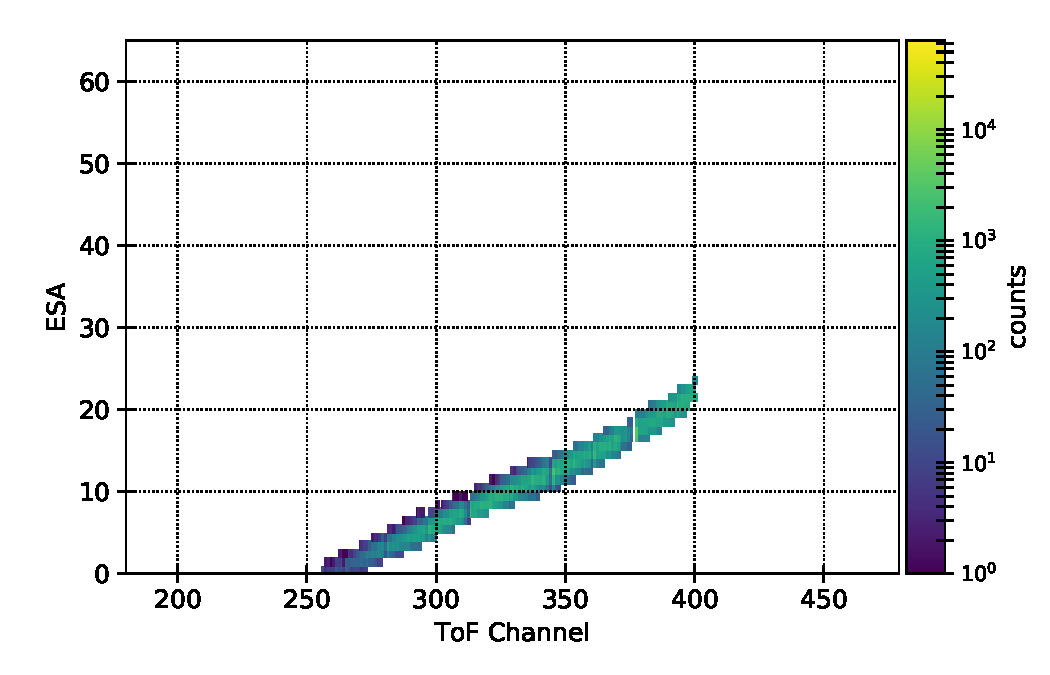
\includegraphics[width=1\linewidth]{Figures/epq_He1.pdf}
	\centering
\end{subfigure}
\begin{subfigure}{.9\linewidth}
	\centering
	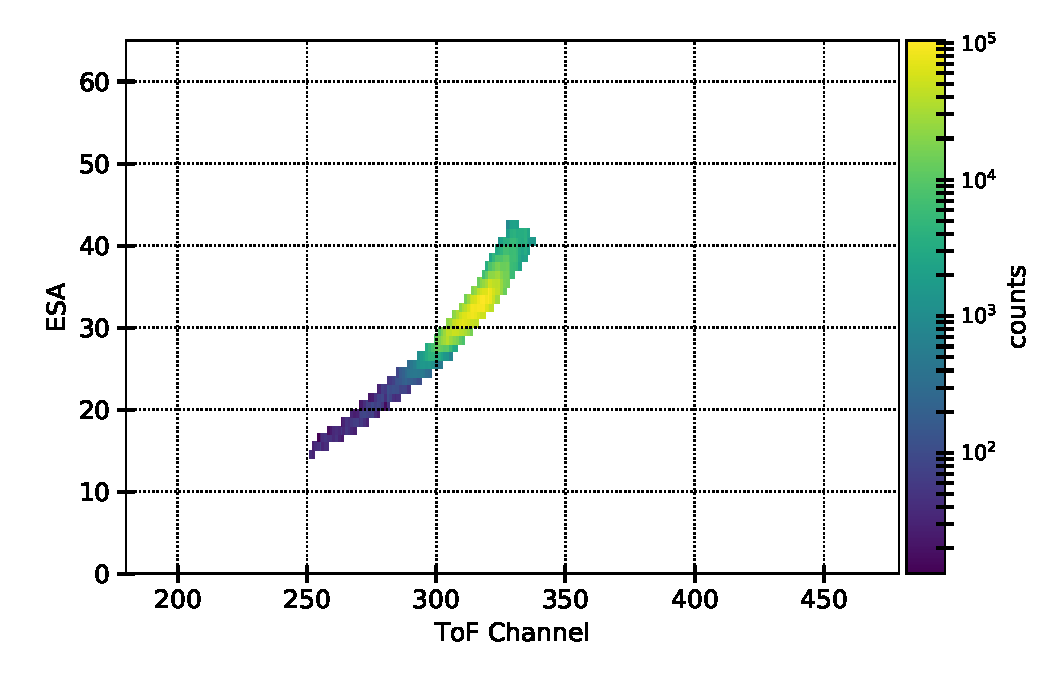
\includegraphics[width=1\linewidth]{Figures/epq_He2.pdf}
	\centering
\end{subfigure}
	\caption{$\mathrm{He^{+}}$ (above) and $\mathrm{He^{2+}}$ (below) selections that have been cut out from fig. \ref{fig:epq_rng0}.}
\label{fig:cutouts}
\end{figure} 
%\include{Chapters/Chapter3}
%\include{Chapters/Chapter4} 
%\include{Chapters/Chapter5} 

%----------------------------------------------------------------------------------------
%	THESIS CONTENT - APPENDICES
%----------------------------------------------------------------------------------------

\appendix % Cue to tell LaTeX that the following "chapters" are Appendices

% Include the appendices of the thesis as separate files from the Appendices folder
% Uncomment the lines as you write the Appendices

% Appendix A

\chapter{Frequently Asked Questions} % Main appendix title

\label{AppendixA} % For referencing this appendix elsewhere, use \ref{AppendixA}

\section{How do I change the colors of links?}

The color of links can be changed to your liking using:

{\small\verb!\hypersetup{urlcolor=red}!}, or

{\small\verb!\hypersetup{citecolor=green}!}, or

{\small\verb!\hypersetup{allcolor=blue}!}.

\noindent If you want to completely hide the links, you can use:

{\small\verb!\hypersetup{allcolors=.}!}, or even better: 

{\small\verb!\hypersetup{hidelinks}!}.

\noindent If you want to have obvious links in the PDF but not the printed text, use:

{\small\verb!\hypersetup{colorlinks=false}!}.

%\include{Appendices/AppendixB}
%\include{Appendices/AppendixC}

%----------------------------------------------------------------------------------------
%	BIBLIOGRAPHY
%----------------------------------------------------------------------------------------

\printbibliography[heading=bibintoc]

%----------------------------------------------------------------------------------------


%----------------------------------------------------------------------------------------
%	DECLARATION PAGE
%----------------------------------------------------------------------------------------

\begin{declaration}
	\addchaptertocentry{\authorshipname} % Add the declaration to the table of contents
	\noindent I, \authorname, declare that this thesis titled,  and the work presented in it are my own. I confirm that:
	
	\begin{itemize} 
		\item This work was done wholly or mainly while in candidature for a research degree at this University.
		\item Where any part of this thesis has previously been submitted for a degree or any other qualification at this University or any other institution, this has been clearly stated.
		\item Where I have consulted the published work of others, this is always clearly attributed.
		\item Where I have quoted from the work of others, the source is always given. With the exception of such quotations, this thesis is entirely my own work.
		\item I have acknowledged all main sources of help.
		\item Where the thesis is based on work done by myself jointly with others, I have made clear exactly what was done by others and what I have contributed myself.\\
	\end{itemize}
	
	\noindent Signed:\\
	\rule[0.5em]{25em}{0.5pt} % This prints a line for the signature
	
	\noindent Date:\\
	\rule[0.5em]{25em}{0.5pt} % This prints a line to write the date
\end{declaration}


%----------------------------------------------------------------------------------------
%	ACKNOWLEDGEMENTS
%----------------------------------------------------------------------------------------

\begin{acknowledgements}
	\addchaptertocentry{\acknowledgementname} % Add the acknowledgements to the table of contents
	The acknowledgments and the people to thank go here, don't forget to include your project advisor\ldots
\end{acknowledgements}


\end{document}  
